\documentclass[11pt]{article}
\usepackage{sectsty}
\allsectionsfont{\color{blue}\fontfamily{lmss}\selectfont}
\usepackage{fontspec}
\setmainfont{XCharter}

\usepackage{listings}
\lstset{
basicstyle=\small\ttfamily,
tabsize=8,
columns=flexible,
breaklines=true,
frame=tb,
rulecolor=\color[rgb]{0.8,0.8,0.7},
backgroundcolor=\color[rgb]{1,1,0.91},
postbreak=\raisebox{0ex}[0ex][0ex]{\ensuremath{\color{red}\hookrightarrow\space}}
}
\usepackage{fontawesome}


\usepackage{mdframed}
\newmdenv[
  backgroundcolor=gray,
  fontcolor=white,
  nobreak=true,
]{terminalinput}



\usepackage{parskip}


    \usepackage[breakable]{tcolorbox}
    \usepackage{parskip} % Stop auto-indenting (to mimic markdown behaviour)

    \usepackage{iftex}
    \ifPDFTeX
    	\usepackage[T1]{fontenc}
    	\usepackage{mathpazo}
    \else
    	\usepackage{fontspec}
    \fi

    % Basic figure setup, for now with no caption control since it's done
    % automatically by Pandoc (which extracts ![](path) syntax from Markdown).
    \usepackage{graphicx}
    % Maintain compatibility with old templates. Remove in nbconvert 6.0
    \let\Oldincludegraphics\includegraphics
    % Ensure that by default, figures have no caption (until we provide a
    % proper Figure object with a Caption API and a way to capture that
    % in the conversion process - todo).
    \usepackage{caption}
    \DeclareCaptionFormat{nocaption}{}
    \captionsetup{format=nocaption,aboveskip=0pt,belowskip=0pt}

    \usepackage{float}
    \floatplacement{figure}{H} % forces figures to be placed at the correct location
    \usepackage{xcolor} % Allow colors to be defined
    \usepackage{enumerate} % Needed for markdown enumerations to work
    \usepackage{geometry} % Used to adjust the document margins
    \usepackage{amsmath} % Equations
    \usepackage{amssymb} % Equations
    \usepackage{textcomp} % defines textquotesingle
    % Hack from http://tex.stackexchange.com/a/47451/13684:
    \AtBeginDocument{%
        \def\PYZsq{\textquotesingle}% Upright quotes in Pygmentized code
    }
    \usepackage{upquote} % Upright quotes for verbatim code
    \usepackage{eurosym} % defines \euro
    \usepackage[mathletters]{ucs} % Extended unicode (utf-8) support
    \usepackage{fancyvrb} % verbatim replacement that allows latex
    \usepackage{grffile} % extends the file name processing of package graphics
                         % to support a larger range
    \makeatletter % fix for old versions of grffile with XeLaTeX
    \@ifpackagelater{grffile}{2019/11/01}
    {
      % Do nothing on new versions
    }
    {
      \def\Gread@@xetex#1{%
        \IfFileExists{"\Gin@base".bb}%
        {\Gread@eps{\Gin@base.bb}}%
        {\Gread@@xetex@aux#1}%
      }
    }
    \makeatother
    \usepackage[Export]{adjustbox} % Used to constrain images to a maximum size
    \adjustboxset{max size={0.9\linewidth}{0.9\paperheight}}

    % The hyperref package gives us a pdf with properly built
    % internal navigation ('pdf bookmarks' for the table of contents,
    % internal cross-reference links, web links for URLs, etc.)
    \usepackage{hyperref}
    % The default LaTeX title has an obnoxious amount of whitespace. By default,
    % titling removes some of it. It also provides customization options.
    \usepackage{titling}
    \usepackage{longtable} % longtable support required by pandoc >1.10
    \usepackage{booktabs}  % table support for pandoc > 1.12.2
    \usepackage[inline]{enumitem} % IRkernel/repr support (it uses the enumerate* environment)
    \usepackage[normalem]{ulem} % ulem is needed to support strikethroughs (\sout)
                                % normalem makes italics be italics, not underlines
    \usepackage{mathrsfs}



    % Colors for the hyperref package
    \definecolor{urlcolor}{rgb}{0,.145,.698}
    \definecolor{linkcolor}{rgb}{.71,0.21,0.01}
    \definecolor{citecolor}{rgb}{.12,.54,.11}

    % ANSI colors
    \definecolor{ansi-black}{HTML}{3E424D}
    \definecolor{ansi-black-intense}{HTML}{282C36}
    \definecolor{ansi-red}{HTML}{E75C58}
    \definecolor{ansi-red-intense}{HTML}{B22B31}
    \definecolor{ansi-green}{HTML}{00A250}
    \definecolor{ansi-green-intense}{HTML}{007427}
    \definecolor{ansi-yellow}{HTML}{DDB62B}
    \definecolor{ansi-yellow-intense}{HTML}{B27D12}
    \definecolor{ansi-blue}{HTML}{208FFB}
    \definecolor{ansi-blue-intense}{HTML}{0065CA}
    \definecolor{ansi-magenta}{HTML}{D160C4}
    \definecolor{ansi-magenta-intense}{HTML}{A03196}
    \definecolor{ansi-cyan}{HTML}{60C6C8}
    \definecolor{ansi-cyan-intense}{HTML}{258F8F}
    \definecolor{ansi-white}{HTML}{C5C1B4}
    \definecolor{ansi-white-intense}{HTML}{A1A6B2}
    \definecolor{ansi-default-inverse-fg}{HTML}{FFFFFF}
    \definecolor{ansi-default-inverse-bg}{HTML}{000000}

    % common color for the border for error outputs.
    \definecolor{outerrorbackground}{HTML}{FFDFDF}

    % commands and environments needed by pandoc snippets
    % extracted from the output of `pandoc -s`
    \providecommand{\tightlist}{%
      \setlength{\itemsep}{0pt}\setlength{\parskip}{0pt}}
    \DefineVerbatimEnvironment{Highlighting}{Verbatim}{commandchars=\\\{\}}
    % Add ',fontsize=\small' for more characters per line
    \newenvironment{Shaded}{}{}
    \newcommand{\KeywordTok}[1]{\textcolor[rgb]{0.00,0.44,0.13}{\textbf{{#1}}}}
    \newcommand{\DataTypeTok}[1]{\textcolor[rgb]{0.56,0.13,0.00}{{#1}}}
    \newcommand{\DecValTok}[1]{\textcolor[rgb]{0.25,0.63,0.44}{{#1}}}
    \newcommand{\BaseNTok}[1]{\textcolor[rgb]{0.25,0.63,0.44}{{#1}}}
    \newcommand{\FloatTok}[1]{\textcolor[rgb]{0.25,0.63,0.44}{{#1}}}
    \newcommand{\CharTok}[1]{\textcolor[rgb]{0.25,0.44,0.63}{{#1}}}
    \newcommand{\StringTok}[1]{\textcolor[rgb]{0.25,0.44,0.63}{{#1}}}
    \newcommand{\CommentTok}[1]{\textcolor[rgb]{0.38,0.63,0.69}{\textit{{#1}}}}
    \newcommand{\OtherTok}[1]{\textcolor[rgb]{0.00,0.44,0.13}{{#1}}}
    \newcommand{\AlertTok}[1]{\textcolor[rgb]{1.00,0.00,0.00}{\textbf{{#1}}}}
    \newcommand{\FunctionTok}[1]{\textcolor[rgb]{0.02,0.16,0.49}{{#1}}}
    \newcommand{\RegionMarkerTok}[1]{{#1}}
    \newcommand{\ErrorTok}[1]{\textcolor[rgb]{1.00,0.00,0.00}{\textbf{{#1}}}}
    \newcommand{\NormalTok}[1]{{#1}}

    % Additional commands for more recent versions of Pandoc
    \newcommand{\ConstantTok}[1]{\textcolor[rgb]{0.53,0.00,0.00}{{#1}}}
    \newcommand{\SpecialCharTok}[1]{\textcolor[rgb]{0.25,0.44,0.63}{{#1}}}
    \newcommand{\VerbatimStringTok}[1]{\textcolor[rgb]{0.25,0.44,0.63}{{#1}}}
    \newcommand{\SpecialStringTok}[1]{\textcolor[rgb]{0.73,0.40,0.53}{{#1}}}
    \newcommand{\ImportTok}[1]{{#1}}
    \newcommand{\DocumentationTok}[1]{\textcolor[rgb]{0.73,0.13,0.13}{\textit{{#1}}}}
    \newcommand{\AnnotationTok}[1]{\textcolor[rgb]{0.38,0.63,0.69}{\textbf{\textit{{#1}}}}}
    \newcommand{\CommentVarTok}[1]{\textcolor[rgb]{0.38,0.63,0.69}{\textbf{\textit{{#1}}}}}
    \newcommand{\VariableTok}[1]{\textcolor[rgb]{0.10,0.09,0.49}{{#1}}}
    \newcommand{\ControlFlowTok}[1]{\textcolor[rgb]{0.00,0.44,0.13}{\textbf{{#1}}}}
    \newcommand{\OperatorTok}[1]{\textcolor[rgb]{0.40,0.40,0.40}{{#1}}}
    \newcommand{\BuiltInTok}[1]{{#1}}
    \newcommand{\ExtensionTok}[1]{{#1}}
    \newcommand{\PreprocessorTok}[1]{\textcolor[rgb]{0.74,0.48,0.00}{{#1}}}
    \newcommand{\AttributeTok}[1]{\textcolor[rgb]{0.49,0.56,0.16}{{#1}}}
    \newcommand{\InformationTok}[1]{\textcolor[rgb]{0.38,0.63,0.69}{\textbf{\textit{{#1}}}}}
    \newcommand{\WarningTok}[1]{\textcolor[rgb]{0.38,0.63,0.69}{\textbf{\textit{{#1}}}}}


    % Define a nice break command that doesn't care if a line doesn't already
    % exist.
    \def\br{\hspace*{\fill} \\* }
    % Math Jax compatibility definitions
    \def\gt{>}
    \def\lt{<}
    \let\Oldtex\TeX
    \let\Oldlatex\LaTeX
    \renewcommand{\TeX}{\textrm{\Oldtex}}
    \renewcommand{\LaTeX}{\textrm{\Oldlatex}}
    % Document parameters
    % Document title
    \title{intro}





% Pygments definitions
\makeatletter
\def\PY@reset{\let\PY@it=\relax \let\PY@bf=\relax%
    \let\PY@ul=\relax \let\PY@tc=\relax%
    \let\PY@bc=\relax \let\PY@ff=\relax}
\def\PY@tok#1{\csname PY@tok@#1\endcsname}
\def\PY@toks#1+{\ifx\relax#1\empty\else%
    \PY@tok{#1}\expandafter\PY@toks\fi}
\def\PY@do#1{\PY@bc{\PY@tc{\PY@ul{%
    \PY@it{\PY@bf{\PY@ff{#1}}}}}}}
\def\PY#1#2{\PY@reset\PY@toks#1+\relax+\PY@do{#2}}

\@namedef{PY@tok@w}{\def\PY@tc##1{\textcolor[rgb]{0.73,0.73,0.73}{##1}}}
\@namedef{PY@tok@c}{\let\PY@it=\textit\def\PY@tc##1{\textcolor[rgb]{0.25,0.50,0.50}{##1}}}
\@namedef{PY@tok@cp}{\def\PY@tc##1{\textcolor[rgb]{0.74,0.48,0.00}{##1}}}
\@namedef{PY@tok@k}{\let\PY@bf=\textbf\def\PY@tc##1{\textcolor[rgb]{0.00,0.50,0.00}{##1}}}
\@namedef{PY@tok@kp}{\def\PY@tc##1{\textcolor[rgb]{0.00,0.50,0.00}{##1}}}
\@namedef{PY@tok@kt}{\def\PY@tc##1{\textcolor[rgb]{0.69,0.00,0.25}{##1}}}
\@namedef{PY@tok@o}{\def\PY@tc##1{\textcolor[rgb]{0.40,0.40,0.40}{##1}}}
\@namedef{PY@tok@ow}{\let\PY@bf=\textbf\def\PY@tc##1{\textcolor[rgb]{0.67,0.13,1.00}{##1}}}
\@namedef{PY@tok@nb}{\def\PY@tc##1{\textcolor[rgb]{0.00,0.50,0.00}{##1}}}
\@namedef{PY@tok@nf}{\def\PY@tc##1{\textcolor[rgb]{0.00,0.00,1.00}{##1}}}
\@namedef{PY@tok@nc}{\let\PY@bf=\textbf\def\PY@tc##1{\textcolor[rgb]{0.00,0.00,1.00}{##1}}}
\@namedef{PY@tok@nn}{\let\PY@bf=\textbf\def\PY@tc##1{\textcolor[rgb]{0.00,0.00,1.00}{##1}}}
\@namedef{PY@tok@ne}{\let\PY@bf=\textbf\def\PY@tc##1{\textcolor[rgb]{0.82,0.25,0.23}{##1}}}
\@namedef{PY@tok@nv}{\def\PY@tc##1{\textcolor[rgb]{0.10,0.09,0.49}{##1}}}
\@namedef{PY@tok@no}{\def\PY@tc##1{\textcolor[rgb]{0.53,0.00,0.00}{##1}}}
\@namedef{PY@tok@nl}{\def\PY@tc##1{\textcolor[rgb]{0.63,0.63,0.00}{##1}}}
\@namedef{PY@tok@ni}{\let\PY@bf=\textbf\def\PY@tc##1{\textcolor[rgb]{0.60,0.60,0.60}{##1}}}
\@namedef{PY@tok@na}{\def\PY@tc##1{\textcolor[rgb]{0.49,0.56,0.16}{##1}}}
\@namedef{PY@tok@nt}{\let\PY@bf=\textbf\def\PY@tc##1{\textcolor[rgb]{0.00,0.50,0.00}{##1}}}
\@namedef{PY@tok@nd}{\def\PY@tc##1{\textcolor[rgb]{0.67,0.13,1.00}{##1}}}
\@namedef{PY@tok@s}{\def\PY@tc##1{\textcolor[rgb]{0.73,0.13,0.13}{##1}}}
\@namedef{PY@tok@sd}{\let\PY@it=\textit\def\PY@tc##1{\textcolor[rgb]{0.73,0.13,0.13}{##1}}}
\@namedef{PY@tok@si}{\let\PY@bf=\textbf\def\PY@tc##1{\textcolor[rgb]{0.73,0.40,0.53}{##1}}}
\@namedef{PY@tok@se}{\let\PY@bf=\textbf\def\PY@tc##1{\textcolor[rgb]{0.73,0.40,0.13}{##1}}}
\@namedef{PY@tok@sr}{\def\PY@tc##1{\textcolor[rgb]{0.73,0.40,0.53}{##1}}}
\@namedef{PY@tok@ss}{\def\PY@tc##1{\textcolor[rgb]{0.10,0.09,0.49}{##1}}}
\@namedef{PY@tok@sx}{\def\PY@tc##1{\textcolor[rgb]{0.00,0.50,0.00}{##1}}}
\@namedef{PY@tok@m}{\def\PY@tc##1{\textcolor[rgb]{0.40,0.40,0.40}{##1}}}
\@namedef{PY@tok@gh}{\let\PY@bf=\textbf\def\PY@tc##1{\textcolor[rgb]{0.00,0.00,0.50}{##1}}}
\@namedef{PY@tok@gu}{\let\PY@bf=\textbf\def\PY@tc##1{\textcolor[rgb]{0.50,0.00,0.50}{##1}}}
\@namedef{PY@tok@gd}{\def\PY@tc##1{\textcolor[rgb]{0.63,0.00,0.00}{##1}}}
\@namedef{PY@tok@gi}{\def\PY@tc##1{\textcolor[rgb]{0.00,0.63,0.00}{##1}}}
\@namedef{PY@tok@gr}{\def\PY@tc##1{\textcolor[rgb]{1.00,0.00,0.00}{##1}}}
\@namedef{PY@tok@ge}{\let\PY@it=\textit}
\@namedef{PY@tok@gs}{\let\PY@bf=\textbf}
\@namedef{PY@tok@gp}{\let\PY@bf=\textbf\def\PY@tc##1{\textcolor[rgb]{0.00,0.00,0.50}{##1}}}
\@namedef{PY@tok@go}{\def\PY@tc##1{\textcolor[rgb]{0.53,0.53,0.53}{##1}}}
\@namedef{PY@tok@gt}{\def\PY@tc##1{\textcolor[rgb]{0.00,0.27,0.87}{##1}}}
\@namedef{PY@tok@err}{\def\PY@bc##1{{\setlength{\fboxsep}{\string -\fboxrule}\fcolorbox[rgb]{1.00,0.00,0.00}{1,1,1}{\strut ##1}}}}
\@namedef{PY@tok@kc}{\let\PY@bf=\textbf\def\PY@tc##1{\textcolor[rgb]{0.00,0.50,0.00}{##1}}}
\@namedef{PY@tok@kd}{\let\PY@bf=\textbf\def\PY@tc##1{\textcolor[rgb]{0.00,0.50,0.00}{##1}}}
\@namedef{PY@tok@kn}{\let\PY@bf=\textbf\def\PY@tc##1{\textcolor[rgb]{0.00,0.50,0.00}{##1}}}
\@namedef{PY@tok@kr}{\let\PY@bf=\textbf\def\PY@tc##1{\textcolor[rgb]{0.00,0.50,0.00}{##1}}}
\@namedef{PY@tok@bp}{\def\PY@tc##1{\textcolor[rgb]{0.00,0.50,0.00}{##1}}}
\@namedef{PY@tok@fm}{\def\PY@tc##1{\textcolor[rgb]{0.00,0.00,1.00}{##1}}}
\@namedef{PY@tok@vc}{\def\PY@tc##1{\textcolor[rgb]{0.10,0.09,0.49}{##1}}}
\@namedef{PY@tok@vg}{\def\PY@tc##1{\textcolor[rgb]{0.10,0.09,0.49}{##1}}}
\@namedef{PY@tok@vi}{\def\PY@tc##1{\textcolor[rgb]{0.10,0.09,0.49}{##1}}}
\@namedef{PY@tok@vm}{\def\PY@tc##1{\textcolor[rgb]{0.10,0.09,0.49}{##1}}}
\@namedef{PY@tok@sa}{\def\PY@tc##1{\textcolor[rgb]{0.73,0.13,0.13}{##1}}}
\@namedef{PY@tok@sb}{\def\PY@tc##1{\textcolor[rgb]{0.73,0.13,0.13}{##1}}}
\@namedef{PY@tok@sc}{\def\PY@tc##1{\textcolor[rgb]{0.73,0.13,0.13}{##1}}}
\@namedef{PY@tok@dl}{\def\PY@tc##1{\textcolor[rgb]{0.73,0.13,0.13}{##1}}}
\@namedef{PY@tok@s2}{\def\PY@tc##1{\textcolor[rgb]{0.73,0.13,0.13}{##1}}}
\@namedef{PY@tok@sh}{\def\PY@tc##1{\textcolor[rgb]{0.73,0.13,0.13}{##1}}}
\@namedef{PY@tok@s1}{\def\PY@tc##1{\textcolor[rgb]{0.73,0.13,0.13}{##1}}}
\@namedef{PY@tok@mb}{\def\PY@tc##1{\textcolor[rgb]{0.40,0.40,0.40}{##1}}}
\@namedef{PY@tok@mf}{\def\PY@tc##1{\textcolor[rgb]{0.40,0.40,0.40}{##1}}}
\@namedef{PY@tok@mh}{\def\PY@tc##1{\textcolor[rgb]{0.40,0.40,0.40}{##1}}}
\@namedef{PY@tok@mi}{\def\PY@tc##1{\textcolor[rgb]{0.40,0.40,0.40}{##1}}}
\@namedef{PY@tok@il}{\def\PY@tc##1{\textcolor[rgb]{0.40,0.40,0.40}{##1}}}
\@namedef{PY@tok@mo}{\def\PY@tc##1{\textcolor[rgb]{0.40,0.40,0.40}{##1}}}
\@namedef{PY@tok@ch}{\let\PY@it=\textit\def\PY@tc##1{\textcolor[rgb]{0.25,0.50,0.50}{##1}}}
\@namedef{PY@tok@cm}{\let\PY@it=\textit\def\PY@tc##1{\textcolor[rgb]{0.25,0.50,0.50}{##1}}}
\@namedef{PY@tok@cpf}{\let\PY@it=\textit\def\PY@tc##1{\textcolor[rgb]{0.25,0.50,0.50}{##1}}}
\@namedef{PY@tok@c1}{\let\PY@it=\textit\def\PY@tc##1{\textcolor[rgb]{0.25,0.50,0.50}{##1}}}
\@namedef{PY@tok@cs}{\let\PY@it=\textit\def\PY@tc##1{\textcolor[rgb]{0.25,0.50,0.50}{##1}}}

\def\PYZbs{\char`\\}
\def\PYZus{\char`\_}
\def\PYZob{\char`\{}
\def\PYZcb{\char`\}}
\def\PYZca{\char`\^}
\def\PYZam{\char`\&}
\def\PYZlt{\char`\<}
\def\PYZgt{\char`\>}
\def\PYZsh{\char`\#}
\def\PYZpc{\char`\%}
\def\PYZdl{\char`\$}
\def\PYZhy{\char`\-}
\def\PYZsq{\char`\'}
\def\PYZdq{\char`\"}
\def\PYZti{\char`\~}
% for compatibility with earlier versions
\def\PYZat{@}
\def\PYZlb{[}
\def\PYZrb{]}
\makeatother


    % For linebreaks inside Verbatim environment from package fancyvrb.
    \makeatletter
        \newbox\Wrappedcontinuationbox
        \newbox\Wrappedvisiblespacebox
        \newcommand*\Wrappedvisiblespace {\textcolor{red}{\textvisiblespace}}
        \newcommand*\Wrappedcontinuationsymbol {\textcolor{red}{\llap{\tiny$\m@th\hookrightarrow$}}}
        \newcommand*\Wrappedcontinuationindent {3ex }
        \newcommand*\Wrappedafterbreak {\kern\Wrappedcontinuationindent\copy\Wrappedcontinuationbox}
        % Take advantage of the already applied Pygments mark-up to insert
        % potential linebreaks for TeX processing.
        %        {, <, #, %, $, ' and ": go to next line.
        %        _, }, ^, &, >, - and ~: stay at end of broken line.
        % Use of \textquotesingle for straight quote.
        \newcommand*\Wrappedbreaksatspecials {%
            \def\PYGZus{\discretionary{\char`\_}{\Wrappedafterbreak}{\char`\_}}%
            \def\PYGZob{\discretionary{}{\Wrappedafterbreak\char`\{}{\char`\{}}%
            \def\PYGZcb{\discretionary{\char`\}}{\Wrappedafterbreak}{\char`\}}}%
            \def\PYGZca{\discretionary{\char`\^}{\Wrappedafterbreak}{\char`\^}}%
            \def\PYGZam{\discretionary{\char`\&}{\Wrappedafterbreak}{\char`\&}}%
            \def\PYGZlt{\discretionary{}{\Wrappedafterbreak\char`\<}{\char`\<}}%
            \def\PYGZgt{\discretionary{\char`\>}{\Wrappedafterbreak}{\char`\>}}%
            \def\PYGZsh{\discretionary{}{\Wrappedafterbreak\char`\#}{\char`\#}}%
            \def\PYGZpc{\discretionary{}{\Wrappedafterbreak\char`\%}{\char`\%}}%
            \def\PYGZdl{\discretionary{}{\Wrappedafterbreak\char`\$}{\char`\$}}%
            \def\PYGZhy{\discretionary{\char`\-}{\Wrappedafterbreak}{\char`\-}}%
            \def\PYGZsq{\discretionary{}{\Wrappedafterbreak\textquotesingle}{\textquotesingle}}%
            \def\PYGZdq{\discretionary{}{\Wrappedafterbreak\char`\"}{\char`\"}}%
            \def\PYGZti{\discretionary{\char`\~}{\Wrappedafterbreak}{\char`\~}}%
        }
        % Some characters . , ; ? ! / are not pygmentized.
        % This macro makes them "active" and they will insert potential linebreaks
        \newcommand*\Wrappedbreaksatpunct {%
            \lccode`\~`\.\lowercase{\def~}{\discretionary{\hbox{\char`\.}}{\Wrappedafterbreak}{\hbox{\char`\.}}}%
            \lccode`\~`\,\lowercase{\def~}{\discretionary{\hbox{\char`\,}}{\Wrappedafterbreak}{\hbox{\char`\,}}}%
            \lccode`\~`\;\lowercase{\def~}{\discretionary{\hbox{\char`\;}}{\Wrappedafterbreak}{\hbox{\char`\;}}}%
            \lccode`\~`\:\lowercase{\def~}{\discretionary{\hbox{\char`\:}}{\Wrappedafterbreak}{\hbox{\char`\:}}}%
            \lccode`\~`\?\lowercase{\def~}{\discretionary{\hbox{\char`\?}}{\Wrappedafterbreak}{\hbox{\char`\?}}}%
            \lccode`\~`\!\lowercase{\def~}{\discretionary{\hbox{\char`\!}}{\Wrappedafterbreak}{\hbox{\char`\!}}}%
            \lccode`\~`\/\lowercase{\def~}{\discretionary{\hbox{\char`\/}}{\Wrappedafterbreak}{\hbox{\char`\/}}}%
            \catcode`\.\active
            \catcode`\,\active
            \catcode`\;\active
            \catcode`\:\active
            \catcode`\?\active
            \catcode`\!\active
            \catcode`\/\active
            \lccode`\~`\~
        }
    \makeatother

    \let\OriginalVerbatim=\Verbatim
    \makeatletter
    \renewcommand{\Verbatim}[1][1]{%
        %\parskip\z@skip
        \sbox\Wrappedcontinuationbox {\Wrappedcontinuationsymbol}%
        \sbox\Wrappedvisiblespacebox {\FV@SetupFont\Wrappedvisiblespace}%
        \def\FancyVerbFormatLine ##1{\hsize\linewidth
            \vtop{\raggedright\hyphenpenalty\z@\exhyphenpenalty\z@
                \doublehyphendemerits\z@\finalhyphendemerits\z@
                \strut ##1\strut}%
        }%
        % If the linebreak is at a space, the latter will be displayed as visible
        % space at end of first line, and a continuation symbol starts next line.
        % Stretch/shrink are however usually zero for typewriter font.
        \def\FV@Space {%
            \nobreak\hskip\z@ plus\fontdimen3\font minus\fontdimen4\font
            \discretionary{\copy\Wrappedvisiblespacebox}{\Wrappedafterbreak}
            {\kern\fontdimen2\font}%
        }%

        % Allow breaks at special characters using \PYG... macros.
        \Wrappedbreaksatspecials
        % Breaks at punctuation characters . , ; ? ! and / need catcode=\active
        \OriginalVerbatim[#1,codes*=\Wrappedbreaksatpunct]%
    }
    \makeatother

    % Exact colors from NB
    \definecolor{incolor}{HTML}{303F9F}
    \definecolor{outcolor}{HTML}{D84315}
    \definecolor{cellborder}{HTML}{CFCFCF}
    \definecolor{cellbackground}{HTML}{F7F7F7}

    % prompt
    \makeatletter
    \newcommand{\boxspacing}{\kern\kvtcb@left@rule\kern\kvtcb@boxsep}
    \makeatother
    \newcommand{\prompt}[4]{
        {\ttfamily\llap{{\color{#2}[#3]:\hspace{3pt}#4}}\vspace{-\baselineskip}}
    }



    % Prevent overflowing lines due to hard-to-break entities
    \sloppy
    % Setup hyperref package
    \hypersetup{
      breaklinks=true,  % so long urls are correctly broken across lines
      colorlinks=true,
      urlcolor=urlcolor,
      linkcolor=linkcolor,
      citecolor=citecolor,
      }
    % Slightly bigger margins than the latex defaults

    \geometry{verbose,tmargin=1in,bmargin=1in,lmargin=1in,rmargin=1in}



\renewcommand{\PY}[2]{{#2}}
\usepackage{fancyhdr}
\pagestyle{fancy}
\rhead{\color{gray}\sf\small\rightmark}
\lhead{\nouppercase{\color{gray}\sf\small\leftmark}}
\cfoot{\color{gray}\sf\thepage}
\renewcommand{\footrulewidth}{1pt}
\begin{document}





    \hypertarget{genome-annotation}{%
\section{Genome Annotation}\label{genome-annotation}}

\hypertarget{introduction}{%
\subsection{Introduction}\label{introduction}}

During the last practical assignment (Genome Assembly), we generated an
assembly of chromosome 5 of the eukaryotic intracellular parasite
\textit{Plasmodium falciparum}. Today we are going to use our assembly to
learn about how to compare different genome assembly versions and
identify sequences that may have some biological function. This process
is known as ``Genome Annotation'' and is graphically represented below:

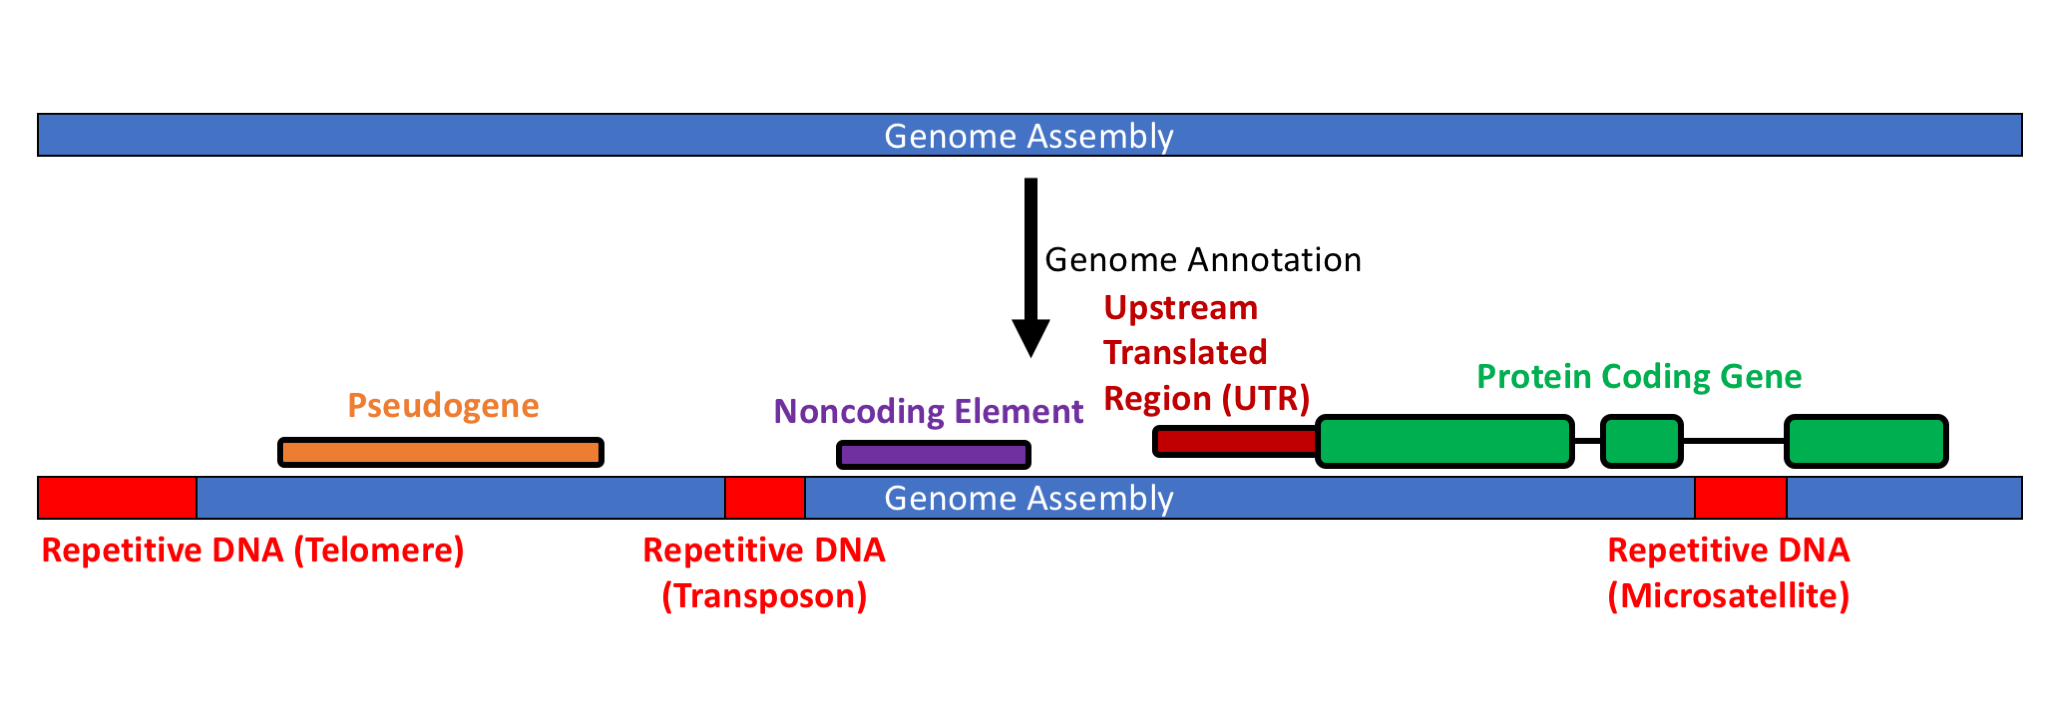
\includegraphics{images/intro_schematic.png}

Genome Annotation is about taking a raw assembled genome (top; like the
one you created in the ``Assembly'' module) and annotating it with
features that biologists are interested in (bottom). While we will not
be annotating all the features outlined above today, this schematic
should give you a general ideal of what this practical is about.

    \hypertarget{learning-outcomes}{%
\subsection{Learning Outcomes}\label{learning-outcomes}}

On completion of the tutorial, you can expect to be able to:

\begin{itemize}
\tightlist
\item
  Align two different reference genome assemblies against one another.
\item
  Identify repetitive DNA sequences.
\item
  Align RNA-seq data to an assembly and use it to identify genes.
\item
  Use comparative genomics to identify similar proteins in other
  organisms.
\end{itemize}

    \hypertarget{tutorial-sections}{%
\subsection{Tutorial sections}\label{tutorial-sections}}

This tutorial comprises the following sections:

\begin{enumerate}
\def\labelenumi{\arabic{enumi}.}
\tightlist
\item
  \href{reference_alignment.ipynb}{Comparing Reference Genomes}
\item
  \href{repetitive_dna.ipynb}{Identifying repetitive DNA}
\item
  \href{gene_discovery.ipynb}{Gene Discovery}
\item
  \href{comparative_genomics.ipynb}{Gene Annotation using Comparative
  Genomics}
\end{enumerate}

    \hypertarget{authors}{%
\subsection{Authors}\label{authors}}

This tutorial was written by
\href{https://github.com/eugenegardner}{Eugene Gardner}.

    \hypertarget{running-the-commands-from-this-tutorial}{%
\subsection{Running the commands from this
tutorial}\label{running-the-commands-from-this-tutorial}}

You can follow this tutorial by typing all the commands you see into a
terminal window. This is similar to the ``Command Prompt'' window on MS
Windows systems, which allows the user to type DOS commands to manage
files.

To get started, open a new terminal window and type the command below:

    \begin{tcolorbox}[breakable, size=fbox, boxrule=1pt, pad at break*=1mm,colback=cellbackground, colframe=cellborder]
\prompt{In}{incolor}{ }{\boxspacing}
\begin{Verbatim}[commandchars=\\\{\}]
\PY{n}{cd} \PY{o}{\PYZti{}}\PY{o}{/}\PY{n}{course\PYZus{}data}\PY{o}{/}\PY{n}{annotation}\PY{o}{/}\PY{n}{data}
\end{Verbatim}
\end{tcolorbox}

    \hypertarget{lets-get-started}{%
\subsection{Let's get started!}\label{lets-get-started}}

This tutorial requires that you have mummer, RepeatMasker, hisat2,
samtools, augustus, and GenomeThreader installed on your computer. These
are already installed on the virtual machine you are using. To check
that these are installed, run the following commands:

    \begin{tcolorbox}[breakable, size=fbox, boxrule=1pt, pad at break*=1mm,colback=cellbackground, colframe=cellborder]
\prompt{In}{incolor}{ }{\boxspacing}
\begin{Verbatim}[commandchars=\\\{\}]
\PY{n}{nucmer}
\PY{n}{RepeatMasker}
\PY{n}{hisat2}
\PY{n}{samtools}
\PY{n}{augustus}
\PY{n}{gth}
\end{Verbatim}
\end{tcolorbox}

    This should return the help message for each of these programs. If you
want to install this software yourself, please see the software
websites:

\begin{itemize}
\tightlist
\item
  the \href{https://github.com/mummer4/mummer}{mummer} website
\item
  the \href{https://www.repeatmasker.org/}{RepeatMasker} website
\item
  the \href{http://daehwankimlab.github.io/hisat2/}{hisat2} website
\item
  the \href{http://www.htslib.org/}{samtools} website
\item
  the \href{https://github.com/Gaius-Augustus/Augustus}{augustus}
  website
\item
  the \href{https://genomethreader.org/}{GenomeThreader} website
\end{itemize}

We also need to add custom scripts to our PATH environmental variable so
that we can run them easily from the command-line. Run the following
command:

    \begin{tcolorbox}[breakable, size=fbox, boxrule=1pt, pad at break*=1mm,colback=cellbackground, colframe=cellborder]
\prompt{In}{incolor}{ }{\boxspacing}
\begin{Verbatim}[commandchars=\\\{\}]
\PY{n}{export} \PY{n}{PATH}\PY{o}{=}\PY{o}{/}\PY{n}{home}\PY{o}{/}\PY{n}{manager}\PY{o}{/}\PY{n}{course\PYZus{}data}\PY{o}{/}\PY{n}{annotation}\PY{o}{/}\PY{n}{scripts}\PY{o}{/}\PY{p}{:}\PY{err}{\PYZdl{}}\PY{n}{PATH}
\end{Verbatim}
\end{tcolorbox}

    Now lets check that you can run the scripts we just added to the path:

    \begin{tcolorbox}[breakable, size=fbox, boxrule=1pt, pad at break*=1mm,colback=cellbackground, colframe=cellborder]
\prompt{In}{incolor}{ }{\boxspacing}
\begin{Verbatim}[commandchars=\\\{\}]
\PY{n}{computeFlankingRegion}\PY{o}{.}\PY{n}{pl}
\PY{n}{augustus}
\end{Verbatim}
\end{tcolorbox}

    Both of these commands should return help information for each program.
If you get an error, close your terminal and restart this tutorial.

Once you have confirmed that you can run all of the above commands,
proceed to \href{reference_alignment.ipynb}{Comparing Reference
Genomes}.


    % Add a bibliography block to the postdoc



\newpage





    \hypertarget{comparing-reference-genomes}{%
\section{Comparing Reference
Genomes}\label{comparing-reference-genomes}}

First, check you are in the correct directory.

    \begin{tcolorbox}[breakable, size=fbox, boxrule=1pt, pad at break*=1mm,colback=cellbackground, colframe=cellborder]
\prompt{In}{incolor}{ }{\boxspacing}
\begin{Verbatim}[commandchars=\\\{\}]
\PY{n}{pwd}
\end{Verbatim}
\end{tcolorbox}

    It should display something like:

\texttt{/home/manager/course\_data/assembly/data}

So, we have done Pacbio and Illumina sequencing, and made a genome
assembly - now what do we do? In many cases, researchers have previously
performed assemblies of a model organism, but these assemblies may be
imperfect due to various factors. Our goal here is to determine how our
reference genome compares to a previous reference genome.

\textbf{Question:} Based on your work during the previous assembly
module, can you a reason why assembly might not be perfect?

    \hypertarget{set-up}{%
\subsection{Set Up}\label{set-up}}

We have already placed a copy of the assembly that you performed
yesterday into your current working directory:

Do the following command to ensure that it is present:

    \begin{tcolorbox}[breakable, size=fbox, boxrule=1pt, pad at break*=1mm,colback=cellbackground, colframe=cellborder]
\prompt{In}{incolor}{ }{\boxspacing}
\begin{Verbatim}[commandchars=\\\{\}]
\PY{n}{ls} \PY{n}{PB}\PY{o}{.}\PY{n}{contigs}\PY{o}{.}\PY{n}{polished}\PY{o}{.}\PY{n}{fasta}
\end{Verbatim}
\end{tcolorbox}

    We first need to convert the header of this file to something that is
easier for our tools to read:

    \begin{tcolorbox}[breakable, size=fbox, boxrule=1pt, pad at break*=1mm,colback=cellbackground, colframe=cellborder]
\prompt{In}{incolor}{ }{\boxspacing}
\begin{Verbatim}[commandchars=\\\{\}]
\PY{p}{\PYZob{}} \PY{n}{echo} \PY{l+s+s2}{\PYZdq{}}\PY{l+s+s2}{\PYZgt{}tig00000001}\PY{l+s+s2}{\PYZdq{}}\PY{p}{;} \PY{n}{tail} \PY{o}{\PYZhy{}}\PY{n}{n}\PY{o}{+}\PY{l+m+mi}{2} \PY{n}{PB}\PY{o}{.}\PY{n}{contigs}\PY{o}{.}\PY{n}{polished}\PY{o}{.}\PY{n}{fasta}\PY{p}{;} \PY{p}{\PYZcb{}} \PY{o}{\PYZgt{}} \PY{n}{PB}\PY{o}{.}\PY{n}{contigs}\PY{o}{.}\PY{n}{polished}\PY{o}{.}\PY{n}{reheader}\PY{o}{.}\PY{n}{fasta}
\end{Verbatim}
\end{tcolorbox}

    You can then run the following command to make sure that you have
performed the formatting correctly:

    \begin{tcolorbox}[breakable, size=fbox, boxrule=1pt, pad at break*=1mm,colback=cellbackground, colframe=cellborder]
\prompt{In}{incolor}{ }{\boxspacing}
\begin{Verbatim}[commandchars=\\\{\}]
\PY{n}{head} \PY{n}{PB}\PY{o}{.}\PY{n}{contigs}\PY{o}{.}\PY{n}{polished}\PY{o}{.}\PY{n}{reheader}\PY{o}{.}\PY{n}{fasta}
\end{Verbatim}
\end{tcolorbox}

    should return something similar to:

\begin{verbatim}
>tig00000001
TCTTATCTTCTTACTCTTATCTTCTTACTTTTCATTTCTTAGTCTTACTTTCTTCTTCTT
ATCTTCTTACTGTTATCTTCTTACTTTTCATTCCTTACTCTTACTTACTTACTCTTATCT
TCTTACTTTTCATTCCTTAGTCTTACTTACTTACTCTTACTTTCTTCTTCTTATCTTCTT
ACTCTTATCTTCTTACTTTTCATTACTTAGTCTTACTTACTTACTCTTACTTACTTACTC
TTATCTTCTTACTTTTCATTCCTTACTCTTACTTACTTACTCTTATCTTCTTACTTTTCA
TTCCTTACTCTTACTTTCTTCTTCTTAGGTCCTTACTTTTAACTTCTTATTCTTACTTTC
TTACTCTTACGTCCTTACTCTTACTTACTTACTCTTATCTTCTTACTTTTCATTCCTTAC
TTTTCATTCCTTACTTTTCATTTCTTCATCTTATCTTCTTACTTTTCATTCCTTACTCTT
ACTTACTTACTCTTATCTTCTTACTTTTCATTTCTTAATCATATATTCTTACTCATATAC
\end{verbatim}

Now index this file so that we can use it for other parts of this
practical:

    \begin{tcolorbox}[breakable, size=fbox, boxrule=1pt, pad at break*=1mm,colback=cellbackground, colframe=cellborder]
\prompt{In}{incolor}{ }{\boxspacing}
\begin{Verbatim}[commandchars=\\\{\}]
\PY{n}{samtools} \PY{n}{faidx} \PY{n}{PB}\PY{o}{.}\PY{n}{contigs}\PY{o}{.}\PY{n}{polished}\PY{o}{.}\PY{n}{reheader}\PY{o}{.}\PY{n}{fasta}
\end{Verbatim}
\end{tcolorbox}

    If these commands did not work, there is a copy of
\texttt{PB.contigs.polished.reheader.fasta} in
\texttt{annotation\_backups/}.

    \hypertarget{visually-comparing-assemblies}{%
\subsection{Visually Comparing
Assemblies}\label{visually-comparing-assemblies}}

Since we know from the Genome Assembly practical that our assembly was
generated from sequencing chromosome 5 of a \textit{P. falciparum}
isolate, we can compare our results to a previously assembled version of
the \textit{P. falciparum} genome. We have pre-downloaded a version of the
current \textit{P. falciparum} reference genome from
\href{https://plasmodb.org}{PlasmoDB} that only contains chromosome 5
and placed it in your current directory. Run the following command to
see what the first 10 lines of the file look like.

    \begin{tcolorbox}[breakable, size=fbox, boxrule=1pt, pad at break*=1mm,colback=cellbackground, colframe=cellborder]
\prompt{In}{incolor}{ }{\boxspacing}
\begin{Verbatim}[commandchars=\\\{\}]
\PY{n}{head} \PY{n}{Pfalc\PYZus{}chr5\PYZus{}ref}\PY{o}{.}\PY{n}{fa}
\end{Verbatim}
\end{tcolorbox}

    This should look similar to your own file that you assembled yesterday.

Next, we are going to use the tool \texttt{mummer} to align our assembly
to the reference sequence of \textit{P. falciparum}. Mummer was developed
to align entire bacterial genomes and is available on both
\href{https://github.com/mummer4/mummer}{github} and through bioconda.
We can align our assembly to the \textit{P. falciparum} reference with the
following command:

    \begin{tcolorbox}[breakable, size=fbox, boxrule=1pt, pad at break*=1mm,colback=cellbackground, colframe=cellborder]
\prompt{In}{incolor}{ }{\boxspacing}
\begin{Verbatim}[commandchars=\\\{\}]
\PY{n}{nucmer} \PY{o}{\PYZhy{}}\PY{n}{p} \PY{n}{aln} \PY{n}{Pfalc\PYZus{}chr5\PYZus{}ref}\PY{o}{.}\PY{n}{fa} \PY{n}{PB}\PY{o}{.}\PY{n}{contigs}\PY{o}{.}\PY{n}{polished}\PY{o}{.}\PY{n}{reheader}\PY{o}{.}\PY{n}{fasta}
\end{Verbatim}
\end{tcolorbox}

    This will generate the file ``aln.delta''. This file contains
information on how the two reference genomes align, but is a difficult
to interpret. Let's generate something that is a bit more
human-readable:

    \begin{tcolorbox}[breakable, size=fbox, boxrule=1pt, pad at break*=1mm,colback=cellbackground, colframe=cellborder]
\prompt{In}{incolor}{ }{\boxspacing}
\begin{Verbatim}[commandchars=\\\{\}]
\PY{n}{show}\PY{o}{\PYZhy{}}\PY{n}{coords} \PY{n}{aln}\PY{o}{.}\PY{n}{delta} \PY{o}{\PYZgt{}} \PY{n}{aln}\PY{o}{.}\PY{n}{coords}
\end{Verbatim}
\end{tcolorbox}

    Let's take a look at the output of \texttt{show-coords} to see if we can
learn anything. Run the following command:

    \begin{tcolorbox}[breakable, size=fbox, boxrule=1pt, pad at break*=1mm,colback=cellbackground, colframe=cellborder]
\prompt{In}{incolor}{ }{\boxspacing}
\begin{Verbatim}[commandchars=\\\{\}]
\PY{n}{head} \PY{n}{aln}\PY{o}{.}\PY{n}{coords}
\end{Verbatim}
\end{tcolorbox}

    You should see a table of information like this:

\begin{verbatim}
   [S1]     [E1] |   [S2]     [E2] | [LEN 1] [LEN 2] | [% IDY] | [TAGS]
=====================================================================================
       1  236439 |       7  236291 |  236439  236285 |   99.87 | PfIT_05    tig00000001
  136356  136443 | 1031955 1031868 |      88      88 |   95.45 | PfIT_05    tig00000001
  136376  136448 |  423822  423750 |      73      73 |  100.00 | PfIT_05    tig00000001
  136376  136447 |  782656  782585 |      72      72 |  100.00 | PfIT_05    tig00000001
  136377  136445 |  862797  862729 |      69      69 |  100.00 | PfIT_05    tig00000001
\end{verbatim}

The S1 and E1 columns represent the START and END coordinates in the
sequence of the genome that you aligned to (so the original Malaria
reference genome) and S2 and E2 represent the START and END coordinates
in the sequence of your assembly (named tig00000001). LEN1 and LEN2
represent the length of the aligned segments and \% IDY is how well the
two sequences match. So a \% IDY of 100 means that the aligned segments
match perfectly.

Now, lets use \texttt{mummerplot} to visualise this result to better
understand what these alignments mean:

    \begin{tcolorbox}[breakable, size=fbox, boxrule=1pt, pad at break*=1mm,colback=cellbackground, colframe=cellborder]
\prompt{In}{incolor}{ }{\boxspacing}
\begin{Verbatim}[commandchars=\\\{\}]
\PY{n}{mummerplot} \PY{o}{\PYZhy{}}\PY{n}{l} \PY{n}{aln}\PY{o}{.}\PY{n}{delta} \PY{o}{\PYZhy{}}\PY{o}{\PYZhy{}}\PY{n}{png}
\end{Verbatim}
\end{tcolorbox}

    We can look at the resulting plot using the default image viewer on your
virtual machine:

    \begin{tcolorbox}[breakable, size=fbox, boxrule=1pt, pad at break*=1mm,colback=cellbackground, colframe=cellborder]
\prompt{In}{incolor}{ }{\boxspacing}
\begin{Verbatim}[commandchars=\\\{\}]
\PY{n}{eog} \PY{n}{out}\PY{o}{.}\PY{n}{png}
\end{Verbatim}
\end{tcolorbox}

    This should give an image like the following:

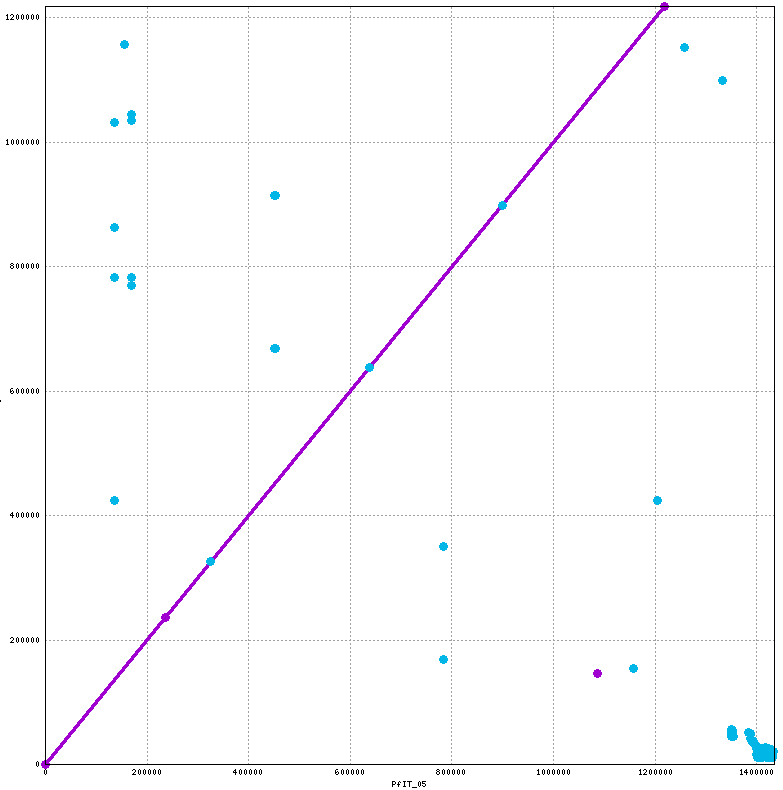
\includegraphics{images/MUMMER_1.png}

The y-axis is our pacbio assembly ordered from position 1 (the bottom)
to position \textasciitilde1,200,000 (the top). The reference \textit{P.
falciparum} genome is on the x-axis. Each place where the two sequences
align perfectly is represented by a purple line. You can see that this
line is right in the middle of the plot, which means that base 10,000 of
our assembly is the same as base 10,000 of the reference, base 40,000 of
our assembly is the same as base 40,000 in the reference, and so on. We
did a good job with our assembly compared to the reference genome!

The blue dots relate to parts of each genome that align multiple times.
In other words, each blue dot is a ``repeat'' in our assembly which
matches the reference more than once.

\textbf{Questions}:

\begin{enumerate}
\def\labelenumi{\arabic{enumi}.}
\tightlist
\item
  Is there an obvious issue with our assembly?
\end{enumerate}

\begin{quote}
\textit{hint: look at the upper right corner of the plot}
\end{quote}

\begin{enumerate}
\def\labelenumi{\arabic{enumi}.}
\setcounter{enumi}{1}
\tightlist
\item
  Why do you think both ends of the reference genome align to the same
  part of our assembled genome?
\end{enumerate}

\begin{quote}
\textit{hint: think about the structure of a chromosome}
\end{quote}

Here is another example of a mummerplot comparing assemblies between two
different isolates of the bacteria H. pylori from the mummer tutorial
website:

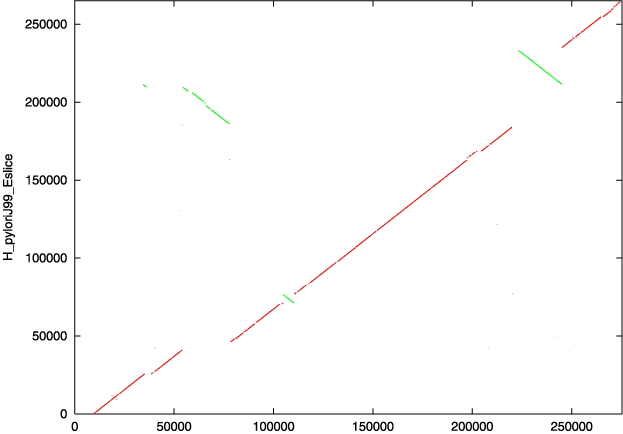
\includegraphics{images/MUMMER_2.png}

\textbf{Questions}:

\begin{enumerate}
\def\labelenumi{\arabic{enumi}.}
\tightlist
\item
  What do you think the green segments represent in this image?
\item
  Why is the red line not centered in the plot and moves up or down?
\end{enumerate}

Now you can move on to \href{repetitive_dna.ipynb}{Repetitive DNA}.


    % Add a bibliography block to the postdoc



\newpage





    \hypertarget{identifying-repetitive-dna}{%
\section{Identifying Repetitive DNA}\label{identifying-repetitive-dna}}

During our previous tutorial on Genome Assembly, we briefly discussed
the problem of repetitive DNA. In the context of genome assembly,
repetitive DNA makes it difficult to piece together separate
``fragments'' to form an entire assembled genome. In this tutorial, we
present repetitive DNA as both a problem and as an interesting
biological question.

    \hypertarget{repetitive-dna}{%
\subsection{Repetitive DNA}\label{repetitive-dna}}

Repetitive DNA comes in many forms. The simplest are long stretches of
identical sequence:

\begin{verbatim}
ATGAGATGACAAAAAAAAAAAAAAAGAGCTGCAGTCCATG
\end{verbatim}

Here, the ``repeat'' is a long stretch of adenine nucleotides. However,
repetitive DNA can also be more complex:

\begin{verbatim}
ATGAGATGACAGAGAGAGAGAGAGAGAGCTGCAGTCCATG
\end{verbatim}

In this case, the repeat is now a two base-pair ``unit'' of adenine and
guanine (AG). We can further increase the complexity:

\begin{verbatim}
TTTAGGGTTCAGGGTTTAGGGTTTAGGGTTCAGGGCTGCAGTCCATG
\end{verbatim}

In this case, the repetitive unit is \texttt{TT(T/C)AGGG}, where
\texttt{(T/C)} means that the 3rd base in the repeat can be
\textit{either} thymine or cytosine. This particular repeat is very
important biologically - it is the repeat at the ends of all \textit{P.
falciparum} chromosomes, or telomeres. You have already seen how
telomeres can affect the ability of researchers to properly assemble
entire genomes in the previous section of this tutorial.

Additionally, some repeats are formed of much larger units and are known
as transposons. These are pieces of DNA that can ``jump'' around the
genome and make new copies of themselves. Transposons can be many
thousands of basepairs long. In \textit{Homo sapiens}, there are three
types of transposons which can still ``jump'': Alu, LINE-1, and SVA.
\textit{P. falciparum}, and in fact all other Apicomplexans, mostly lack
transposons, so we do not have to worry about them as part of this
practical. If you want to read more on tranposons, this paper is a great
place to start:

Henry L. Levin and John V. Moran. \textit{\textbf{Dynamic interactions
between transposable elements and their hosts}}. Nature Reviews Genetics
(2011).

Please note that this section is not an exhaustive list of all possible
DNA repeats. For further reading on how repetitive DNA can effect genome
assembly and annotation, a good place to start is:

Todd J. Treangen and Steven L. Salzberg. \textit{\textbf{Repetitive DNA
and next-generation sequencing: computational challenges and
solutions}}. Nature Reviews Genetics (2011).

    \hypertarget{exercise}{%
\subsection{Exercise}\label{exercise}}

Here is a piece of DNA from \textit{P. falciparum}. Can you identify
repetitive DNA sequences that are longer than 5 base pairs in this
sequence?

\begin{verbatim}
TATAAATACAATATAATATAACGACGAACAGATATGAAAGTGTTAGAACTAGACATACCA
TTTTTCTGTGAAAAATACTTCAAGCTGTAGTATTATTATTATTGCGCTGCTTAGATGTAGT
\end{verbatim}

\textbf{Question:} Can you think of any problems that a Malaria genome
may cause when searching for repeats?

\begin{quote}
\textit{hint: look at part 5 from the ``Genome Assembly'' tutorial}
\end{quote}

    \hypertarget{masking-a-genome}{%
\subsection{Masking a Genome}\label{masking-a-genome}}

The most widely used approach to identify repetitive DNA is called
``RepeatMasker''. Arian Smit \textit{et al.} developed the RepeatMasker
algorithm in the 1990s to identify repeats in the large amount of
sequencing data that was being produced at the time. RepeatMasker
utilizes a statistical method known as a ``Hidden Markov Model'' or HMM
to accurately identify repetitive DNA. The methodology behind HMMs is
beyond the scope of this course, but if you want to learn more
\href{https://towardsdatascience.com/hidden-markov-model-hmm-simple-explanation-in-high-level-b8722fa1a0d5}{this
website} is a good, simple introduction.

Before we can perform annotation, we now need to identify repetitive DNA
that may confuse the tools we will use later today. To do this, we will
use the RepeatMasker tool discussed above. RepeatMasker is preinstalled
on your VM, but is available
\href{https://www.repeatmasker.org/}{online}.

Here, we are going to run ``RepeatMasker'' to ``mask'' our assembled
genome. In the case of genome annotation, to ``mask'' simply means to
identify repetitive DNA. In this tutorial, we are going to change any
letter in our genome fasta file from \texttt{UPPER\ CASE} to
\texttt{lower\ case} where we think there is a repeat. This allows
programs like ``Augustus'' (which we will use later) to identify DNA
repeats and avoid them if necessary.

To run RepeatMasker, just do:

    \begin{tcolorbox}[breakable, size=fbox, boxrule=1pt, pad at break*=1mm,colback=cellbackground, colframe=cellborder]
\prompt{In}{incolor}{ }{\boxspacing}
\begin{Verbatim}[commandchars=\\\{\}]
\PY{n}{RepeatMasker} \PY{o}{\PYZhy{}}\PY{n}{species} \PY{n}{plasmodium} \PY{o}{\PYZhy{}}\PY{n}{xsmall} \PY{n}{PB}\PY{o}{.}\PY{n}{contigs}\PY{o}{.}\PY{n}{polished}\PY{o}{.}\PY{n}{reheader}\PY{o}{.}\PY{n}{fasta}
\end{Verbatim}
\end{tcolorbox}

    \begin{itemize}
\tightlist
\item
  \texttt{-species\ plasmodium} tells RepeatMasker to use a HMM trained
  on \textit{Plasmodium} species.
\item
  \texttt{-xsmall} tells RepeatMasker to write lower case letters of
  masked sequences.
\end{itemize}

This command should take a few minutes and generate three files. You can
see them with the following command:

    \begin{tcolorbox}[breakable, size=fbox, boxrule=1pt, pad at break*=1mm,colback=cellbackground, colframe=cellborder]
\prompt{In}{incolor}{ }{\boxspacing}
\begin{Verbatim}[commandchars=\\\{\}]
\PY{n}{ls} \PY{n}{PB}\PY{o}{.}\PY{n}{contigs}\PY{o}{.}\PY{n}{polished}\PY{o}{.}\PY{n}{reheader}\PY{o}{.}\PY{n}{fasta}\PY{o}{.}\PY{o}{*}
\end{Verbatim}
\end{tcolorbox}

    which should return something like:

\begin{verbatim}
PB.contigs.polished.reheader.fasta.masked
PB.contigs.polished.reheader.fasta.out
PB.contigs.polished.reheader.fasta.tbl
\end{verbatim}

\begin{itemize}
\tightlist
\item
  \texttt{PB.contigs.polished.reheader.fasta.out} contains an extensive
  list of all the repeats ``masked'' in our assembled genome
\item
  \texttt{PB.contigs.polished.reheader.fasta.masked} is the exact same
  as \texttt{PB.contigs.polished.reheader.fasta} except with all of
  those repeats in lower-case letters.
\item
  \texttt{PB.contigs.polished.reheader.fasta.tbl} contains more specific
  information and numbers on what was masked.
\end{itemize}

Look at the contents of \texttt{PB.contigs.polished.reheader.fasta.tbl}
to answer the following questions (use \texttt{more}, \texttt{less} or
\texttt{cat}):

\textbf{Questions:}

\begin{enumerate}
\def\labelenumi{\arabic{enumi}.}
\tightlist
\item
  Why do the sections ``Retroelements'' and ``DNA transposons'' all have
  zeros?
\item
  Approximately what proportion of our genome assembly was masked?
\end{enumerate}

Now let's rename \texttt{PB.contigs.polished.reheader.fasta.masked} to a
shorter name to make it easier to use later:

    \begin{tcolorbox}[breakable, size=fbox, boxrule=1pt, pad at break*=1mm,colback=cellbackground, colframe=cellborder]
\prompt{In}{incolor}{ }{\boxspacing}
\begin{Verbatim}[commandchars=\\\{\}]
\PY{n}{mv} \PY{n}{PB}\PY{o}{.}\PY{n}{contigs}\PY{o}{.}\PY{n}{polished}\PY{o}{.}\PY{n}{reheader}\PY{o}{.}\PY{n}{fasta}\PY{o}{.}\PY{n}{masked} \PY{n}{PB}\PY{o}{.}\PY{n}{masked}\PY{o}{.}\PY{n}{fasta}
\end{Verbatim}
\end{tcolorbox}

    and then index it:

    \begin{tcolorbox}[breakable, size=fbox, boxrule=1pt, pad at break*=1mm,colback=cellbackground, colframe=cellborder]
\prompt{In}{incolor}{ }{\boxspacing}
\begin{Verbatim}[commandchars=\\\{\}]
\PY{n}{samtools} \PY{n}{faidx} \PY{n}{PB}\PY{o}{.}\PY{n}{masked}\PY{o}{.}\PY{n}{fasta}
\end{Verbatim}
\end{tcolorbox}

    If RepeatMasker did not work properly or took too long to run, we have
placed a backup masked genome at:

\texttt{assembly\_backups/PB.masked.fasta}

Once you have masked your genome, move on to
\href{gene_discovery.ipynb}{Gene Discovery}


    % Add a bibliography block to the postdoc



\newpage





    \hypertarget{finding-genes}{%
\section{Finding Genes}\label{finding-genes}}

Now that we have run RepeatMasker on our assembled genome, we are going
to identify coding genes. To do this, we can generally take a few
different approaches:

\begin{enumerate}
\def\labelenumi{\arabic{enumi}.}
\item
  Using RNA-seq data that we generated for our organism, which we can
  align to the genome, and then use it to identify genes.
\item
  Using another similar organism for which we already have information
  on what genes should ``look like''. For example, we can use already
  identified human genes to identify genes in a chimpanzee genome.
\end{enumerate}

Today, we are going to use the first approach. In this section we are
going to use RNA-seq data to identify genes in four basic steps:

\begin{enumerate}
\def\labelenumi{\arabic{enumi}.}
\tightlist
\item
  Align RNA-seq data to our assembly.
\item
  Identify putative introns in these alignments.
\item
  Train a model that tells Augustus what a gene in our assembly looks
  like.
\item
  Identify genes with Augustus.
\end{enumerate}

    \hypertarget{aligning-rna-seq-data}{%
\subsection{Aligning RNA-seq data}\label{aligning-rna-seq-data}}

For our input RNA-seq data we are going to use sequencing generated by a
\textit{P. falciparum} project performed in part at the Wellcome Sanger
Institute in Cambridge, UK. We are going to use this data to help us
build a model of what a gene in our assembled genome should look like.
This data comes from the following paper:

Lia Chappell, Philipp Ross, Lindsey Orchard, Timothy J. Russell, Thomas
D. Otto, Matthew Berriman, Julian C. Rayner, and Manuel Llinás.
\textit{\textbf{Refining the transcriptome of the human malaria parasite
Plasmodium falciparum using amplification-free RNA-seq}}. BMC Genomics,
2020.

To generate the data used by this module, we accessed the sequencing
data generated by the above paper on the
\href{https://www.ebi.ac.uk/ena/browser/home}{European Nucleotide
Archive} under the accession \texttt{ERX2287076}. This accession
represents paired-end Illumina-based short-read sequencing data
generated for a single \textit{P. falciparum} isolate. We have already
filtered the reads to those which should align to the assembly that you
generated as part of the assembly module.

Take a look at the data in your terminal:

    \begin{tcolorbox}[breakable, size=fbox, boxrule=1pt, pad at break*=1mm,colback=cellbackground, colframe=cellborder]
\prompt{In}{incolor}{ }{\boxspacing}
\begin{Verbatim}[commandchars=\\\{\}]
\PY{n}{zcat} \PY{n}{Pfalc\PYZus{}chr5}\PY{o}{.}\PY{l+m+mf}{1.}\PY{n}{fq}\PY{o}{.}\PY{n}{gz} \PY{o}{|} \PY{n}{head} \PY{o}{\PYZhy{}}\PY{n}{n} \PY{l+m+mi}{12}
\end{Verbatim}
\end{tcolorbox}

    This command should show you the first 3 reads in this file.

You should have already learned how to align RNA-seq data as part of the
RNA-seq module. We are going to use the same approach but for our
assembly.

First, we have to index our assembly we made yesterday. This command
makes it suitable for RNA-seq alignment with \texttt{hisat2}:

    \begin{tcolorbox}[breakable, size=fbox, boxrule=1pt, pad at break*=1mm,colback=cellbackground, colframe=cellborder]
\prompt{In}{incolor}{ }{\boxspacing}
\begin{Verbatim}[commandchars=\\\{\}]
\PY{n}{hisat2}\PY{o}{\PYZhy{}}\PY{n}{build} \PY{n}{PB}\PY{o}{.}\PY{n}{masked}\PY{o}{.}\PY{n}{fasta} \PY{n}{PB}\PY{o}{.}\PY{n}{masked}\PY{o}{.}\PY{n}{fasta}\PY{o}{.}\PY{n}{idx}
\end{Verbatim}
\end{tcolorbox}

    Now we are going to align our reads to our reference genome:

    \begin{tcolorbox}[breakable, size=fbox, boxrule=1pt, pad at break*=1mm,colback=cellbackground, colframe=cellborder]
\prompt{In}{incolor}{ }{\boxspacing}
\begin{Verbatim}[commandchars=\\\{\}]
\PY{n}{hisat2} \PY{o}{\PYZhy{}}\PY{o}{\PYZhy{}}\PY{n+nb}{max}\PY{o}{\PYZhy{}}\PY{n}{intronlen} \PY{l+m+mi}{10000} \PY{o}{\PYZhy{}}\PY{n}{x} \PY{n}{PB}\PY{o}{.}\PY{n}{masked}\PY{o}{.}\PY{n}{fasta}\PY{o}{.}\PY{n}{idx} \PY{o}{\PYZhy{}}\PY{l+m+mi}{1} \PY{n}{Pfalc\PYZus{}chr5}\PY{o}{.}\PY{l+m+mf}{1.}\PY{n}{fq}\PY{o}{.}\PY{n}{gz} \PY{o}{\PYZhy{}}\PY{l+m+mi}{2} \PY{n}{Pfalc\PYZus{}chr5}\PY{o}{.}\PY{l+m+mf}{2.}\PY{n}{fq}\PY{o}{.}\PY{n}{gz} \PY{o}{\PYZgt{}} \PY{n}{Pfalc}\PY{o}{.}\PY{n}{sam}
\end{Verbatim}
\end{tcolorbox}

    Now, convert the alignment to bam:

    \begin{tcolorbox}[breakable, size=fbox, boxrule=1pt, pad at break*=1mm,colback=cellbackground, colframe=cellborder]
\prompt{In}{incolor}{ }{\boxspacing}
\begin{Verbatim}[commandchars=\\\{\}]
\PY{n}{samtools} \PY{n}{view} \PY{o}{\PYZhy{}}\PY{n}{Sbo} \PY{n}{Pfalc}\PY{o}{.}\PY{n}{bam} \PY{n}{Pfalc}\PY{o}{.}\PY{n}{sam}
\end{Verbatim}
\end{tcolorbox}

    Our gene finding approach that we will perform later requires an extra
processing step. This tool will filter out alignments that align to our
assembly more than once:

    \begin{tcolorbox}[breakable, size=fbox, boxrule=1pt, pad at break*=1mm,colback=cellbackground, colframe=cellborder]
\prompt{In}{incolor}{ }{\boxspacing}
\begin{Verbatim}[commandchars=\\\{\}]
\PY{n}{filterBam} \PY{o}{\PYZhy{}}\PY{o}{\PYZhy{}}\PY{n}{uniq} \PY{o}{\PYZhy{}}\PY{o}{\PYZhy{}}\PY{o+ow}{in} \PY{n}{Pfalc}\PY{o}{.}\PY{n}{bam} \PY{o}{\PYZhy{}}\PY{o}{\PYZhy{}}\PY{n}{out} \PY{n}{Pfalc}\PY{o}{.}\PY{n}{ssf}\PY{o}{.}\PY{n}{bam} \PY{o}{\PYZhy{}}\PY{o}{\PYZhy{}}\PY{n}{paired} \PY{o}{\PYZhy{}}\PY{o}{\PYZhy{}}\PY{n}{pairwiseAlignment}
\end{Verbatim}
\end{tcolorbox}

    The \texttt{-\/-paired} and \texttt{-\/-pairwiseAlignment} tags tell
\texttt{filterBam} that we are using paired-end data.

Now we sort and index the file as we did in the RNA-seq module:

    \begin{tcolorbox}[breakable, size=fbox, boxrule=1pt, pad at break*=1mm,colback=cellbackground, colframe=cellborder]
\prompt{In}{incolor}{ }{\boxspacing}
\begin{Verbatim}[commandchars=\\\{\}]
\PY{n}{samtools} \PY{n}{sort} \PY{o}{\PYZhy{}}\PY{n}{o} \PY{n}{Pfalc}\PY{o}{.}\PY{n}{sorted}\PY{o}{.}\PY{n}{ssf}\PY{o}{.}\PY{n}{bam} \PY{n}{Pfalc}\PY{o}{.}\PY{n}{ssf}\PY{o}{.}\PY{n}{bam}

\PY{n}{samtools} \PY{n}{index} \PY{n}{Pfalc}\PY{o}{.}\PY{n}{sorted}\PY{o}{.}\PY{n}{ssf}\PY{o}{.}\PY{n}{bam}
\end{Verbatim}
\end{tcolorbox}

    We will take a look at these reads in IGV later to see how well our
alignment worked.

We are now ready to start gene discovery.

    \hypertarget{converting-rna-seq-data-to-intron-information}{%
\subsection{Converting RNA-seq data to intron
information}\label{converting-rna-seq-data-to-intron-information}}

We are now going to start using the Augustus tool. Augustus is available
on github:

https://github.com/Gaius-Augustus/Augustus

Augustus was originally published as a free web-tool in the following
paper:

Mario Stanke and Burkhard Morgenstern. \textit{\textbf{AUGUSTUS: a web
server for gene prediction in eukaryotes that allows user-defined
constraints}}. Nucleic Acids Research (2005).

To find genes, Augustus needs information on what a gene ``looks like''
in the organism that you have assembled. In Eukaryotic genomes (such as
\textit{P. falciparum}), the most complicated part of gene discovery
typically is identifying introns/splice sites. Augustus thus uses the
RNA-seq data we generated above to identify patterns in the DNA sequence
which are indicative of splicing.

This practical follows several parts of a tutorial developed by the
Augustus authors which was published as part of the following paper:

Katharina J. Hoff and Mario Stanke. \textit{\textbf{Predicting Genes in
Single Genomes with AUGUSTUS}}. Current Protocols in Bioinformatics
(2018).

A free preprint of this publication, which is very similar to the
published version, is available using
\href{https://math-inf.uni-greifswald.de/storages/uni-greifswald/fakultaet/mnf/mathinf/stanke/augustus_wrp.pdf}{this
link}.

This workflow also makes use of several scripts from the tool BRAKER,
also written by the Augustus authors. We have copied the scripts
required for this tutorial from BRAKER's
\href{https://github.com/Gaius-Augustus/BRAKER}{github repository} for
you to use today and placed them in the
\texttt{\textasciitilde{}/course\_data/annotation/scripts/} folder.

\textbf{Please note:} The method presented here is a simplification of
the approach that you would need to take to accurately predict genes in
a new genome and is presented here as a foundation on which to build. We
have omitted several steps for the sake of computing resources and time.
See the above Augustus tutorial for further steps that can be taken to
more accurately predict genes in genome assemblies. There are other
tools and resources that can be used to annotate both eukaryotic and
prokaryotic genomes.

First, we need to find all the introns in our aligned RNA-sequencing
data and then filter out low-quality introns:

    \begin{tcolorbox}[breakable, size=fbox, boxrule=1pt, pad at break*=1mm,colback=cellbackground, colframe=cellborder]
\prompt{In}{incolor}{ }{\boxspacing}
\begin{Verbatim}[commandchars=\\\{\}]
\PY{n}{bam2hints} \PY{o}{\PYZhy{}}\PY{o}{\PYZhy{}}\PY{n}{intronsonly} \PY{o}{\PYZhy{}}\PY{o}{\PYZhy{}}\PY{o+ow}{in}\PY{o}{=}\PY{n}{Pfalc}\PY{o}{.}\PY{n}{sorted}\PY{o}{.}\PY{n}{ssf}\PY{o}{.}\PY{n}{bam} \PY{o}{\PYZhy{}}\PY{o}{\PYZhy{}}\PY{n}{out}\PY{o}{=}\PY{n}{Pfalc}\PY{o}{.}\PY{n}{introns}\PY{o}{.}\PY{n}{gff}

\PY{n}{filterIntronsFindStrand}\PY{o}{.}\PY{n}{pl} \PY{n}{PB}\PY{o}{.}\PY{n}{masked}\PY{o}{.}\PY{n}{fasta} \PY{n}{Pfalc}\PY{o}{.}\PY{n}{introns}\PY{o}{.}\PY{n}{gff} \PY{o}{\PYZhy{}}\PY{o}{\PYZhy{}}\PY{n}{score} \PY{o}{\PYZgt{}} \PY{n}{Pfalc}\PY{o}{.}\PY{n}{introns}\PY{o}{.}\PY{n}{f}\PY{o}{.}\PY{n}{gff}
\end{Verbatim}
\end{tcolorbox}

    Next, we would normally use the
\href{http://exon.gatech.edu/GeneMark/gmes_instructions.html}{``GeneMark-ES''}
software to identify genes using our intron predictions. Unfortunately,
the licence of GeneMark-ES prevents us from putting this software on a
virtual machine. As such, we have pre-run ``GeneMark-ES'' on the data in
this module and provided the necessary output for you already in the
file \texttt{genemark.gtf}.

To generate this file we used the following command (Do not run this
command!):

    \begin{tcolorbox}[breakable, size=fbox, boxrule=1pt, pad at break*=1mm,colback=cellbackground, colframe=cellborder]
\prompt{In}{incolor}{ }{\boxspacing}
\begin{Verbatim}[commandchars=\\\{\}]
\PY{n}{gmes\PYZus{}petap}\PY{o}{.}\PY{n}{pl} \PY{o}{\PYZhy{}}\PY{o}{\PYZhy{}}\PY{n}{verbose} \PY{o}{\PYZhy{}}\PY{o}{\PYZhy{}}\PY{n}{sequence}\PY{o}{=}\PY{n}{PB}\PY{o}{.}\PY{n}{masked}\PY{o}{.}\PY{n}{fasta} \PY{o}{\PYZhy{}}\PY{o}{\PYZhy{}}\PY{n}{ET}\PY{o}{=}\PY{n}{Pfalc}\PY{o}{.}\PY{n}{introns}\PY{o}{.}\PY{n}{f}\PY{o}{.}\PY{n}{gff} \PY{o}{\PYZhy{}}\PY{o}{\PYZhy{}}\PY{n}{soft\PYZus{}mask} \PY{l+m+mi}{1000}
\end{Verbatim}
\end{tcolorbox}

    While we cannot demonstrate how this code runs today, you can go to the
\href{http://exon.gatech.edu/GeneMark/gmes_instructions.html}{GeneMark-ES
website} and download a copy for your own personal use after this
course.

Let's take a look at the output of GeneMark-ES and see what it contains:

    \begin{tcolorbox}[breakable, size=fbox, boxrule=1pt, pad at break*=1mm,colback=cellbackground, colframe=cellborder]
\prompt{In}{incolor}{ }{\boxspacing}
\begin{Verbatim}[commandchars=\\\{\}]
\PY{n}{head} \PY{o}{\PYZhy{}}\PY{n}{n} \PY{l+m+mi}{31} \PY{n}{genemark}\PY{o}{.}\PY{n}{gtf}
\end{Verbatim}
\end{tcolorbox}

    This command should print predictions for the first two genes identified
by GeneMark-ES, fittingly named ``1\_g'' and ``2\_g''.

\textbf{Questions:}

\begin{enumerate}
\def\labelenumi{\arabic{enumi}.}
\tightlist
\item
  How many exons does the gene ``1\_g'' have?
\item
  Can you think of a simple LINUX command to figure out how many genes
  GeneMark-ES identified?
\item
  How many genes did GeneMark find?
\end{enumerate}

Next, we are going to use various commands from
\href{https://github.com/Gaius-Augustus/BRAKER}{BRAKER} to generate a
list of ``high quality'' genes using the list of introns
(\texttt{Pfalc.introns.f.gff}) and gene predictions from GeneMark-ES
(\texttt{genemark.gtf}) that you made above:

    \begin{tcolorbox}[breakable, size=fbox, boxrule=1pt, pad at break*=1mm,colback=cellbackground, colframe=cellborder]
\prompt{In}{incolor}{ }{\boxspacing}
\begin{Verbatim}[commandchars=\\\{\}]
\PY{n}{filterGenemark}\PY{o}{.}\PY{n}{pl} \PY{n}{genemark}\PY{o}{.}\PY{n}{gtf} \PY{n}{Pfalc}\PY{o}{.}\PY{n}{introns}\PY{o}{.}\PY{n}{f}\PY{o}{.}\PY{n}{gff}
\end{Verbatim}
\end{tcolorbox}

    This command will generate two files: \texttt{genemark.f.good.gtf} and
\texttt{genemark.f.bad.gtf} that we will use later.

This command should also give output like (actual output may differ
slightly):

\begin{verbatim}
Number of cds hints is 0
Average gene length: 2614
Average number of introns: 1.89261744966443
Good gene rate: 0.422818791946309
Number of genes: 300
Number of complete genes: 298
Number of good genes: 126
Number of one-exon-genes: 104
Number of bad genes: 174
Good intron rate: 0.200570201421801
One exon gene rate (of good genes): 0.349206349206349
One exon gene rate (of all genes): 0.346666666666667
\end{verbatim}

This output is telling us that, out of the total number of genes
predicted by GeneMark-ES (300), only 126 look like real genes according
to Augustus.

Next, we are going to use scripts provided as part of Augustus to
further filter our predicted genes down to a set of reliable hits. Run
the following command:

    \begin{tcolorbox}[breakable, size=fbox, boxrule=1pt, pad at break*=1mm,colback=cellbackground, colframe=cellborder]
\prompt{In}{incolor}{ }{\boxspacing}
\begin{Verbatim}[commandchars=\\\{\}]
\PY{n}{computeFlankingRegion}\PY{o}{.}\PY{n}{pl} \PY{n}{genemark}\PY{o}{.}\PY{n}{f}\PY{o}{.}\PY{n}{good}\PY{o}{.}\PY{n}{gtf}
\end{Verbatim}
\end{tcolorbox}

    This command is simply calculating the total length of genes from our
predictions above. It should generate an output similar to:

\begin{verbatim}
Total length gene length (including introns): 220281. Number of genes: 321.
Average Length: 686.233644859813

The flanking_DNA value is: 343 (the Minimum of 10 000 and 343)
\end{verbatim}

This is telling us that our predicted genes are, on average, about 670
basepairs long. We now need to use the value provided by this script, or
approximately half the mean gene length (343) in our following commands:

    \begin{tcolorbox}[breakable, size=fbox, boxrule=1pt, pad at break*=1mm,colback=cellbackground, colframe=cellborder]
\prompt{In}{incolor}{ }{\boxspacing}
\begin{Verbatim}[commandchars=\\\{\}]
\PY{n}{gff2gbSmallDNA}\PY{o}{.}\PY{n}{pl} \PY{n}{genemark}\PY{o}{.}\PY{n}{gtf} \PY{n}{PB}\PY{o}{.}\PY{n}{masked}\PY{o}{.}\PY{n}{fasta} \PY{l+m+mi}{343} \PY{n}{tmp}\PY{o}{.}\PY{n}{gb} \PY{l+m+mi}{2}\PY{o}{\PYZgt{}} \PY{o}{/}\PY{n}{dev}\PY{o}{/}\PY{n}{null}

\PY{n}{filterGenesIn\PYZus{}mRNAname}\PY{o}{.}\PY{n}{pl} \PY{n}{genemark}\PY{o}{.}\PY{n}{f}\PY{o}{.}\PY{n}{good}\PY{o}{.}\PY{n}{gtf} \PY{n}{tmp}\PY{o}{.}\PY{n}{gb} \PY{o}{\PYZgt{}} \PY{n}{bonafide}\PY{o}{.}\PY{n}{gb}
\end{Verbatim}
\end{tcolorbox}

    This will generate our list of likely true genes (\texttt{bonafide.gb})
so that we can get to identifying actual genes in our assembly. This
file is in ``genbank'' format, the same format used by NCBI's GenBank to
store sequence data about genes. You can go to GenBank with the
following link: https://www.ncbi.nlm.nih.gov/genbank/

\textbf{Questions:}

\begin{enumerate}
\def\labelenumi{\arabic{enumi}.}
\tightlist
\item
  What is the part of the command \texttt{2\textgreater{}\ /dev/null}
  actually doing?
\item
  How many genes are in our final set of possible genes
  (\texttt{bonafide.gb})?
\end{enumerate}

We are now ready to train Augustus to actually find genes. If these
commands did not work, we have placed a backup of \texttt{bonafide.gb}
in the \texttt{annotation\_backups/} folder.

    \hypertarget{training-augustus-for-gene-finding}{%
\subsection{Training Augustus for Gene
Finding}\label{training-augustus-for-gene-finding}}

We are now going to use our set of likely genes to ``train'' augustus on
what a gene in our \textit{P. falciparum} assembly looks like. This
approach uses a test-training method, where we split our genes into two
pieces and ``train'' augustus on one half, and ``test'' on the other.

This approach allows us to remove statistical circularity. In other
words, we can see how good our predictor is since we don't use our
testing set to train the data.

We have already created some files in the \texttt{species/} directory
for you to use for this exercise. But we first need to tell augustus
that this directory is where we want our training data to go:

    \begin{tcolorbox}[breakable, size=fbox, boxrule=1pt, pad at break*=1mm,colback=cellbackground, colframe=cellborder]
\prompt{In}{incolor}{ }{\boxspacing}
\begin{Verbatim}[commandchars=\\\{\}]
\PY{n}{export} \PY{n}{AUGUSTUS\PYZus{}CONFIG\PYZus{}PATH}\PY{o}{=}\PY{o}{/}\PY{n}{home}\PY{o}{/}\PY{n}{manager}\PY{o}{/}\PY{n}{course\PYZus{}data}\PY{o}{/}\PY{n}{annotation}\PY{o}{/}\PY{n}{data}\PY{o}{/}
\end{Verbatim}
\end{tcolorbox}

    This is known in linux as setting an ``environment variable''. This
allows programs (like Augustus) to know certain pieces of information
when they run. You can see that the environment variable is set properly
by typing:

    \begin{tcolorbox}[breakable, size=fbox, boxrule=1pt, pad at break*=1mm,colback=cellbackground, colframe=cellborder]
\prompt{In}{incolor}{ }{\boxspacing}
\begin{Verbatim}[commandchars=\\\{\}]
\PY{n}{echo} \PY{err}{\PYZdl{}}\PY{n}{AUGUSTUS\PYZus{}CONFIG\PYZus{}PATH}
\end{Verbatim}
\end{tcolorbox}

    This should print the same path that we set above.

We can now tell Augustus that we are going to train a new model, and
Augustus will automatically place default files in the directory
\texttt{species/mygenome/}:

    \begin{tcolorbox}[breakable, size=fbox, boxrule=1pt, pad at break*=1mm,colback=cellbackground, colframe=cellborder]
\prompt{In}{incolor}{ }{\boxspacing}
\begin{Verbatim}[commandchars=\\\{\}]
\PY{n}{new\PYZus{}species}\PY{o}{.}\PY{n}{pl} \PY{o}{\PYZhy{}}\PY{o}{\PYZhy{}}\PY{n}{species}\PY{o}{=}\PY{n}{mygenome}

\PY{n}{etraining} \PY{o}{\PYZhy{}}\PY{o}{\PYZhy{}}\PY{n}{species}\PY{o}{=}\PY{n}{mygenome} \PY{n}{bonafide}\PY{o}{.}\PY{n}{gb}
\end{Verbatim}
\end{tcolorbox}

    You can put any name for \texttt{-\/-species}, but for today we will use
``mygenome''. The first command sets up a working directory, and the
second does an initial round of training on our genes. After running
this command run the following:

    \begin{tcolorbox}[breakable, size=fbox, boxrule=1pt, pad at break*=1mm,colback=cellbackground, colframe=cellborder]
\prompt{In}{incolor}{ }{\boxspacing}
\begin{Verbatim}[commandchars=\\\{\}]
\PY{n}{ls} \PY{n}{species}\PY{o}{/}\PY{n}{mygenome}\PY{o}{/}
\end{Verbatim}
\end{tcolorbox}

    You should see the following output:

\begin{verbatim}
mygenome_exon_probs.pbl    mygenome_intron_probs.pbl  mygenome_metapars.cgp.cfg
mygenome_parameters.cfg    mygenome_igenic_probs.pbl  mygenome_metapars.cfg
mygenome_metapars.utr.cfg  mygenome_weightmatrix.txt
\end{verbatim}

These files contain information Augustus needs to identify genes. We are
now going to identify better parameters using our test/training
approach. First, we need to make a test and training set like we
described above. In this case, we are going to simply split our data in
half. But how many genes is that? To find out how many genes we have do:

    \begin{tcolorbox}[breakable, size=fbox, boxrule=1pt, pad at break*=1mm,colback=cellbackground, colframe=cellborder]
\prompt{In}{incolor}{ }{\boxspacing}
\begin{Verbatim}[commandchars=\\\{\}]
\PY{n}{grep} \PY{o}{\PYZhy{}}\PY{n}{c} \PY{n}{LOCUS} \PY{n}{bonafide}\PY{o}{.}\PY{n}{gb}
\end{Verbatim}
\end{tcolorbox}

    This should give ``126'' (if it doesn't don't worry, just change the
following accordingly). So, if we are going to split 50/50 to form
train/test sets, we need to put 63 genes in both our training and test
set (126 / 2 = 63). The following command will do this for us:

    \begin{tcolorbox}[breakable, size=fbox, boxrule=1pt, pad at break*=1mm,colback=cellbackground, colframe=cellborder]
\prompt{In}{incolor}{ }{\boxspacing}
\begin{Verbatim}[commandchars=\\\{\}]
\PY{n}{randomSplit}\PY{o}{.}\PY{n}{pl} \PY{n}{bonafide}\PY{o}{.}\PY{n}{gb} \PY{l+m+mi}{63}
\end{Verbatim}
\end{tcolorbox}

    This will create two files: \texttt{bonafide.gb.train} and
\texttt{bonafide.gb.test}.

Now, lets run training on our training set:

    \begin{tcolorbox}[breakable, size=fbox, boxrule=1pt, pad at break*=1mm,colback=cellbackground, colframe=cellborder]
\prompt{In}{incolor}{ }{\boxspacing}
\begin{Verbatim}[commandchars=\\\{\}]
\PY{n}{etraining} \PY{o}{\PYZhy{}}\PY{o}{\PYZhy{}}\PY{n}{species}\PY{o}{=}\PY{n}{mygenome} \PY{n}{bonafide}\PY{o}{.}\PY{n}{gb}\PY{o}{.}\PY{n}{train} \PY{o}{\PYZam{}}\PY{o}{\PYZgt{}} \PY{n}{etrain}\PY{o}{.}\PY{n}{out}
\end{Verbatim}
\end{tcolorbox}

    What new information did this teach us? Most importantly, it gave us
information on how often different stop codons are used. We can get this
information from the ``tail'' of the output file with the following
command:

    \begin{tcolorbox}[breakable, size=fbox, boxrule=1pt, pad at break*=1mm,colback=cellbackground, colframe=cellborder]
\prompt{In}{incolor}{ }{\boxspacing}
\begin{Verbatim}[commandchars=\\\{\}]
\PY{n}{tail} \PY{o}{\PYZhy{}}\PY{n}{n} \PY{l+m+mi}{6} \PY{n}{etrain}\PY{o}{.}\PY{n}{out}
\end{Verbatim}
\end{tcolorbox}

    This command simply prints the last 6 lines of this file, and you should
see something like:

\begin{verbatim}
tag:    7 (0.111)
taa:   40 (0.635)
tga:   16 (0.254)
end *EXON*
Storing parameters to file...
Writing exon model parameters [1] to file
/home/manager/course_data/annotation/data/species/mygenome/mygenome_exon_probs.pbl.
\end{verbatim}

This command takes care of most of the training, but we need to manually
adjust a few parameters on our own. We are going to use a text editor
known as \texttt{gedit} to change the training parameters according to
the above data. Open the file we need to change:

    \begin{tcolorbox}[breakable, size=fbox, boxrule=1pt, pad at break*=1mm,colback=cellbackground, colframe=cellborder]
\prompt{In}{incolor}{ }{\boxspacing}
\begin{Verbatim}[commandchars=\\\{\}]
\PY{n}{gedit} \PY{n}{species}\PY{o}{/}\PY{n}{mygenome}\PY{o}{/}\PY{n}{mygenome\PYZus{}parameters}\PY{o}{.}\PY{n}{cfg}
\end{Verbatim}
\end{tcolorbox}

    Now find the lines by scrolling through the file our using ``find''
(ctrl+f) that look like:

\begin{verbatim}
/Constant/amberprob                   0.33   # Prob(stop codon = tag), if 0 tag is assumed to ...
/Constant/ochreprob                   0.33   # Prob(stop codon = taa), if 0 taa is assumed to ...
/Constant/opalprob                    0.34   # Prob(stop codon = tga), if 0 tga is assumed to ...
\end{verbatim}

And change them to match the output of our command above, like:

\begin{verbatim}
/Constant/amberprob                   0.111   # Prob(stop codon = tag), if 0 tag is assumed to ...
/Constant/ochreprob                   0.635   # Prob(stop codon = taa), if 0 taa is assumed to ...
/Constant/opalprob                    0.254   # Prob(stop codon = tga), if 0 tga is assumed to ...
\end{verbatim}

Make sure you \textit{save} the file before exiting - by using either the
``Save'' button at the top-right or by hitting ``ctrl+s'' on your
keyboard.

Finally, we are going to run Augustus on our test set and see how good
our prediction is!

    \begin{tcolorbox}[breakable, size=fbox, boxrule=1pt, pad at break*=1mm,colback=cellbackground, colframe=cellborder]
\prompt{In}{incolor}{ }{\boxspacing}
\begin{Verbatim}[commandchars=\\\{\}]
\PY{n}{augustus} \PY{o}{\PYZhy{}}\PY{o}{\PYZhy{}}\PY{n}{species}\PY{o}{=}\PY{n}{mygenome} \PY{n}{junk}\PY{o}{/}\PY{n}{bonafide}\PY{o}{.}\PY{n}{gb}\PY{o}{.}\PY{n}{test} \PY{o}{\PYZgt{}} \PY{n}{test}\PY{o}{.}\PY{n}{out}
\end{Verbatim}
\end{tcolorbox}

    So, how did we do? The last 41 lines of the file \texttt{test.out} tell
us exactly how well we did:

    \begin{tcolorbox}[breakable, size=fbox, boxrule=1pt, pad at break*=1mm,colback=cellbackground, colframe=cellborder]
\prompt{In}{incolor}{ }{\boxspacing}
\begin{Verbatim}[commandchars=\\\{\}]
\PY{n}{tail} \PY{o}{\PYZhy{}}\PY{n}{n} \PY{l+m+mi}{41} \PY{n}{test}\PY{o}{.}\PY{n}{out}
\end{Verbatim}
\end{tcolorbox}

    This file provides 4 different tables, 1 for each of:

\begin{enumerate}
\def\labelenumi{\arabic{enumi}.}
\tightlist
\item
  Nucleotide-level prediction - are individual bases predicted to be
  part of genes, found within genes?
\item
  Exon-level prediction - are individual exons predicted properly?
\item
  Transcript-level prediction - are entire transcripts predicted
  properly?
\item
  UTR-based prediction - We didn't train our approach for UTRs, ignore
  this table
\end{enumerate}

For each, we get different statistics, but let's focus on sensitivity
and specificity. These two values are commonly used in test-training
approaches and in machine learning like the one we have used here. For
our exon level data, we should have a table similar to this:

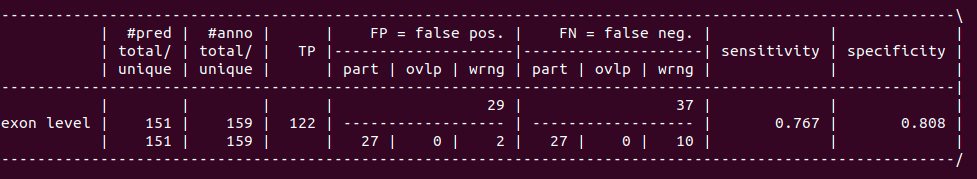
\includegraphics{images/gene_1.png}

Now what do these values mean in plain English:

\begin{itemize}
\tightlist
\item
  Sensitivity - How did we do in identifying real exons?

  \begin{itemize}
  \tightlist
  \item
    Out of the total number of actual true exons (159), we found 110
    total true events:

    \begin{itemize}
    \tightlist
    \item
      110/159 = 69.2\%
    \end{itemize}
  \end{itemize}
\item
  Specificity - How many exons did we identify that are not real exons?

  \begin{itemize}
  \tightlist
  \item
    Out of the total number of predictions (144), we found 34 additional
    events that are not actually exons:

    \begin{itemize}
    \tightlist
    \item
      1 - (34 / 144) = 76.4\%
    \end{itemize}
  \end{itemize}
\end{itemize}

Overall, this is a pretty good start for identifying exons. You may have
noticed in one of the other tables that our ability to predict entire
transcripts is not nearly as good. We will visually evalute the results
at the end of this section to see why that may be.

\textbf{Question:} What do you think a limitation of using just 1
chromosome to train our gene finder is?

    \hypertarget{identifying-genes}{%
\subsection{Identifying Genes}\label{identifying-genes}}

Let's quickly review what we have done:

\begin{enumerate}
\def\labelenumi{\arabic{enumi}.}
\tightlist
\item
  Aligned RNA-seq data to our assembly
\item
  Identified putative introns in these alignments
\item
  Trained a model that tells Augustus what a gene in our assembly looks
  like.
\end{enumerate}

So, all that is left is to:

\begin{enumerate}
\def\labelenumi{\arabic{enumi}.}
\setcounter{enumi}{3}
\tightlist
\item
  Identify genes
\end{enumerate}

Now to actually run Augustus on our assembly:

    \begin{tcolorbox}[breakable, size=fbox, boxrule=1pt, pad at break*=1mm,colback=cellbackground, colframe=cellborder]
\prompt{In}{incolor}{ }{\boxspacing}
\begin{Verbatim}[commandchars=\\\{\}]
\PY{n}{augustus} \PY{o}{\PYZhy{}}\PY{o}{\PYZhy{}}\PY{n}{species}\PY{o}{=}\PY{n}{mygenome} \PY{n}{PB}\PY{o}{.}\PY{n}{masked}\PY{o}{.}\PY{n}{fasta} \PY{o}{\PYZgt{}} \PY{n}{PB}\PY{o}{.}\PY{n}{contigs}\PY{o}{.}\PY{n}{gff}
\end{Verbatim}
\end{tcolorbox}

    This command will likely take a minute or two depending on the computer
you are using.

We are also going to run Augustus using their default parameters,
trained for \textit{P. falciparum}, to compare against:

    \begin{tcolorbox}[breakable, size=fbox, boxrule=1pt, pad at break*=1mm,colback=cellbackground, colframe=cellborder]
\prompt{In}{incolor}{ }{\boxspacing}
\begin{Verbatim}[commandchars=\\\{\}]
\PY{n}{augustus} \PY{o}{\PYZhy{}}\PY{o}{\PYZhy{}}\PY{n}{species}\PY{o}{=}\PY{n}{pfalciparum} \PY{n}{PB}\PY{o}{.}\PY{n}{masked}\PY{o}{.}\PY{n}{fasta} \PY{o}{\PYZgt{}} \PY{n}{PB}\PY{o}{.}\PY{n}{contigs}\PY{o}{.}\PY{n}{default}\PY{o}{.}\PY{n}{gff}
\end{Verbatim}
\end{tcolorbox}

    Each of these commands will generate a single gff format file. The
ENSEMBL website has more information on the format of
\href{https://www.ensembl.org/info/website/upload/gff.html}{gff files}.

\textbf{Questions:}

\begin{enumerate}
\def\labelenumi{\arabic{enumi}.}
\tightlist
\item
  Can you figure out how many genes each approach found?
\item
  We identified protein coding genes, but can you think of any other
  types of annotations we could find with Augustus?
\end{enumerate}

\begin{quote}
\textit{hint: look back at the introduction to this practical.}
\end{quote}

    \hypertarget{checking-our-annotations-in-igv}{%
\subsection{Checking our Annotations in
IGV}\label{checking-our-annotations-in-igv}}

Now that we have some genes, lets use the
\href{https://software.broadinstitute.org/software/igv/}{Integrative
Genomics Viewer} to explore our results. You should have used IGV as
part of several of the modules of this course, including RNA-seq and
CHIP-seq. We will be using a similar approach here.

Go ahead and open IGV:

    \begin{tcolorbox}[breakable, size=fbox, boxrule=1pt, pad at break*=1mm,colback=cellbackground, colframe=cellborder]
\prompt{In}{incolor}{ }{\boxspacing}
\begin{Verbatim}[commandchars=\\\{\}]
\PY{n}{igv} \PY{o}{\PYZam{}}
\end{Verbatim}
\end{tcolorbox}

    The \texttt{\&} symbol tells IGV to open in another window on your
virtual machine's desktop, but allows you to continue using your
terminal. We are going to load your assembly as a genome in IGV.

Now, load your assembly, RNA-seq alignments, and gene data into IGV:

\begin{enumerate}
\def\labelenumi{\arabic{enumi}.}
\tightlist
\item
  \textbf{Go to \textit{``Genomes -\textgreater{} Load Genome From
  File\ldots{}''}. Select ``PB.masked.fasta'' and click
  \textit{``Open''}.}
\item
  \textbf{Go to \textit{``File -\textgreater{} Load From File''}. Select
  ``Pfalc.sorted.ssf.bam'' and click \textit{``Open''}.}
\item
  \textbf{Go to \textit{``File -\textgreater{} Load From File''}. Select
  ``PB.contigs.gff'' and click \textit{``Open''}.}
\item
  \textbf{Go to \textit{``File -\textgreater{} Load From File''}. Select
  ``PB.contigs.default.gff'' and click \textit{``Open''}.}
\end{enumerate}

You should now have your assembly loaded into IGV, a set of RNA-seq
reads labeled ``Pfalc.sorted.bam Coverage'' and ``Pfalc.sorted.bam'' and
two gene annotations. Make sure you ``\textit{right click}'' on the gene
annotation and click \textit{``Squished''} so that you can see exon-intron
information. Your window should look like:

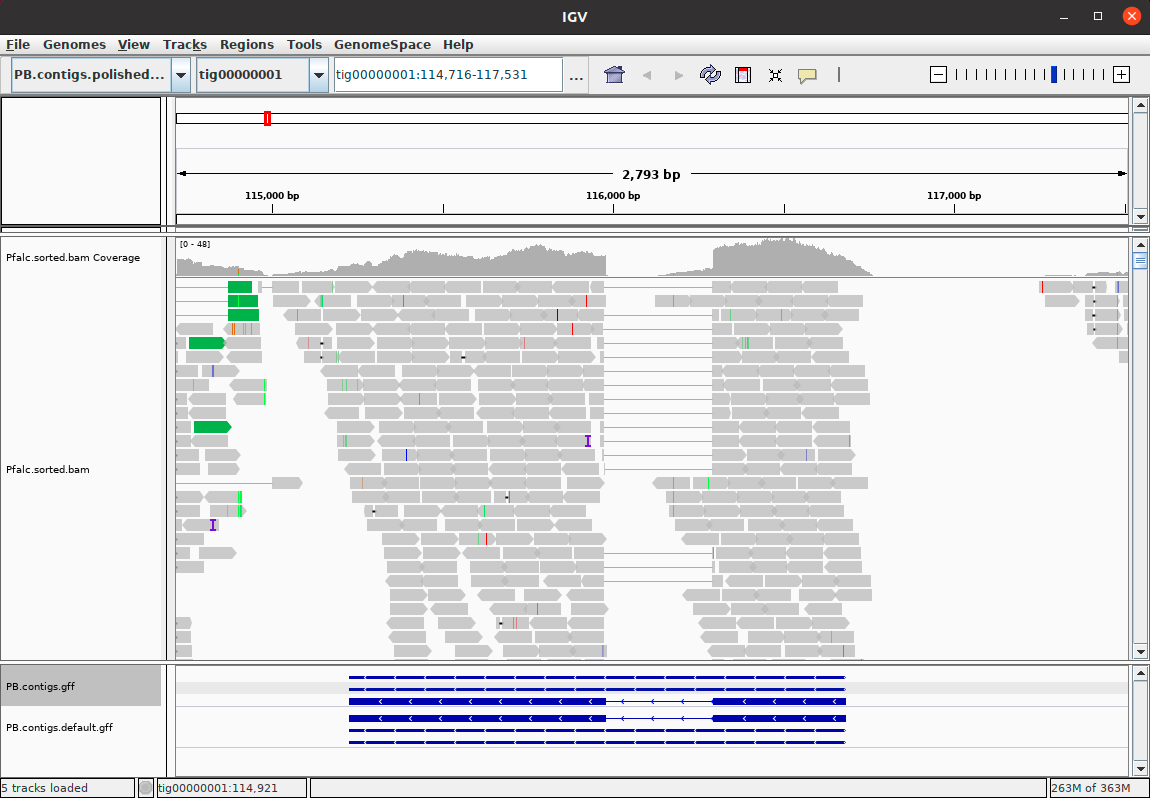
\includegraphics{images/IGV_1.png}

Now, navigate to the top of the window and go to the coordinates:

\begin{verbatim}
tig00000001:77,000-80,500
\end{verbatim}

\textbf{Questions:}

\begin{enumerate}
\def\labelenumi{\arabic{enumi}.}
\tightlist
\item
  How many exons does this gene have?
\item
  Do you think there are any issues in the gene structure?
\item
  How do the predictions for your model versus the default model
  compare?
\end{enumerate}

Now go to the coordinates:

\begin{verbatim}
tig00000001:123,400-126,800
\end{verbatim}

\textbf{Questions:}

\begin{enumerate}
\def\labelenumi{\arabic{enumi}.}
\tightlist
\item
  What is the main difference between your genes and the default genes?
\item
  Does the default make sense, why?
\item
  What are both predictions missing, and why do you think that is?
\end{enumerate}

\begin{quote}
\textit{hint: look back at the introduction to this practical.}
\end{quote}

Finally, go to the coordinates:

\begin{verbatim}
tig00000001:165,000-171,500
\end{verbatim}

If you click on the gene structure (the one with exons and introns) of
the gene in IGV, you should see a window like the following:

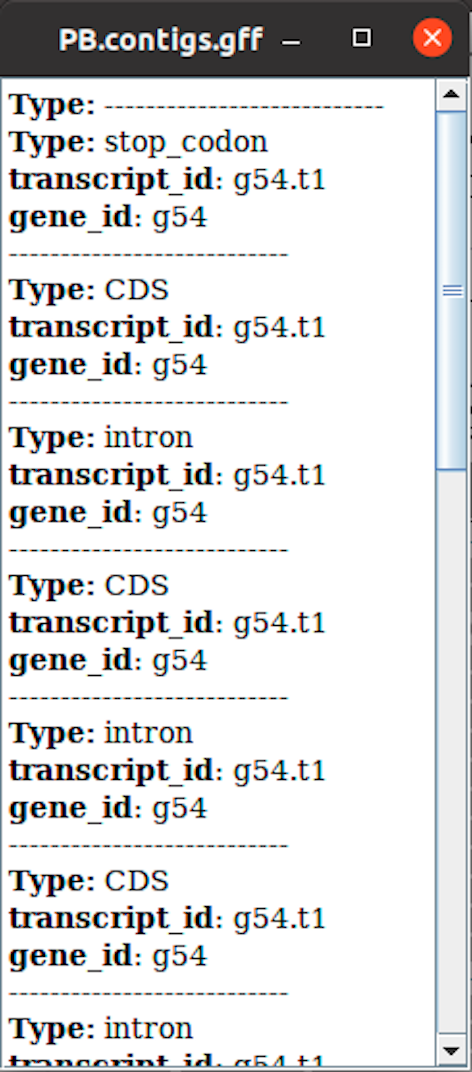
\includegraphics{images/IGV_2.png}

The ``name'' of this gene in the window is g54, which simply means that
it is the 54th gene that Augustus identified. Note that the name of your
gene may be slightly different - please adjust the following commands
accordingly. We can then go back to our terminal and find this gene in
our .gff file using a simple command like grep:

    \begin{tcolorbox}[breakable, size=fbox, boxrule=1pt, pad at break*=1mm,colback=cellbackground, colframe=cellborder]
\prompt{In}{incolor}{ }{\boxspacing}
\begin{Verbatim}[commandchars=\\\{\}]
\PY{n}{grep} \PY{o}{\PYZhy{}}\PY{n}{A} \PY{l+m+mi}{30} \PY{l+s+s2}{\PYZdq{}}\PY{l+s+s2}{start gene g54}\PY{l+s+s2}{\PYZdq{}} \PY{n}{PB}\PY{o}{.}\PY{n}{contigs}\PY{o}{.}\PY{n}{gff}
\end{Verbatim}
\end{tcolorbox}

    \begin{itemize}
\tightlist
\item
  \texttt{-A} tells us how many lines ``after'' we match g54 we should
  report.
\end{itemize}

Make sure to modify your command if the gene is not named ``g54''. Note
that this command will not work for every gene that we identified
exactly as written as they will have a different length (modifiable with
the \texttt{-A} parameter) and a different name.

\textbf{Questions:}

\begin{enumerate}
\def\labelenumi{\arabic{enumi}.}
\tightlist
\item
  How many exons does this gene have?
\item
  How many introns?
\item
  How can you extract the same information for another gene by modifying
  the above command? Report the command and result here.
\end{enumerate}

Feel free to explore the data in IGV before you continue to the final
module, \href{comparative_genomics.ipynb}{Comparative Genomics}.


    % Add a bibliography block to the postdoc



\newpage





    \hypertarget{using-comparative-genomics-to-identify-genes}{%
\section{Using Comparative Genomics to Identify
Genes}\label{using-comparative-genomics-to-identify-genes}}

We have predicted some genes, but what does this actually do for us?
Biologically, we want to assign a function to genes so that we can try
to understand what they are doing. Now, we are going to use an alignment
approach to assign a biological function to genes that we predicted.

In the previous section, we identified genes on one chromosome of
\textit{P. falciparum}. \textit{P. falciparum} has been extensively studied,
and a large proportion of the genes in its genome have been assigned
some function. However, lets pretend that the genes we just identified
are from a new exciting organism that we just sequenced, and we want to
find out a potential function for these genes. In many cases, an
organism that is relatively closely related to the one that we are
interested in has already been sequenced, and gene discovery as outlined
above has already been performed. Here is a phylogenetic tree of
different \textit{Plasmodium} species from the paper:

M. Andreina Pacheco et. al.~\textit{\textbf{Malarial parasite diversity in
chimpanzees: The value of comparative approaches to ascertain the
evolution of Plasmodium falciparum antigens}}. Malaria Journal (2013).

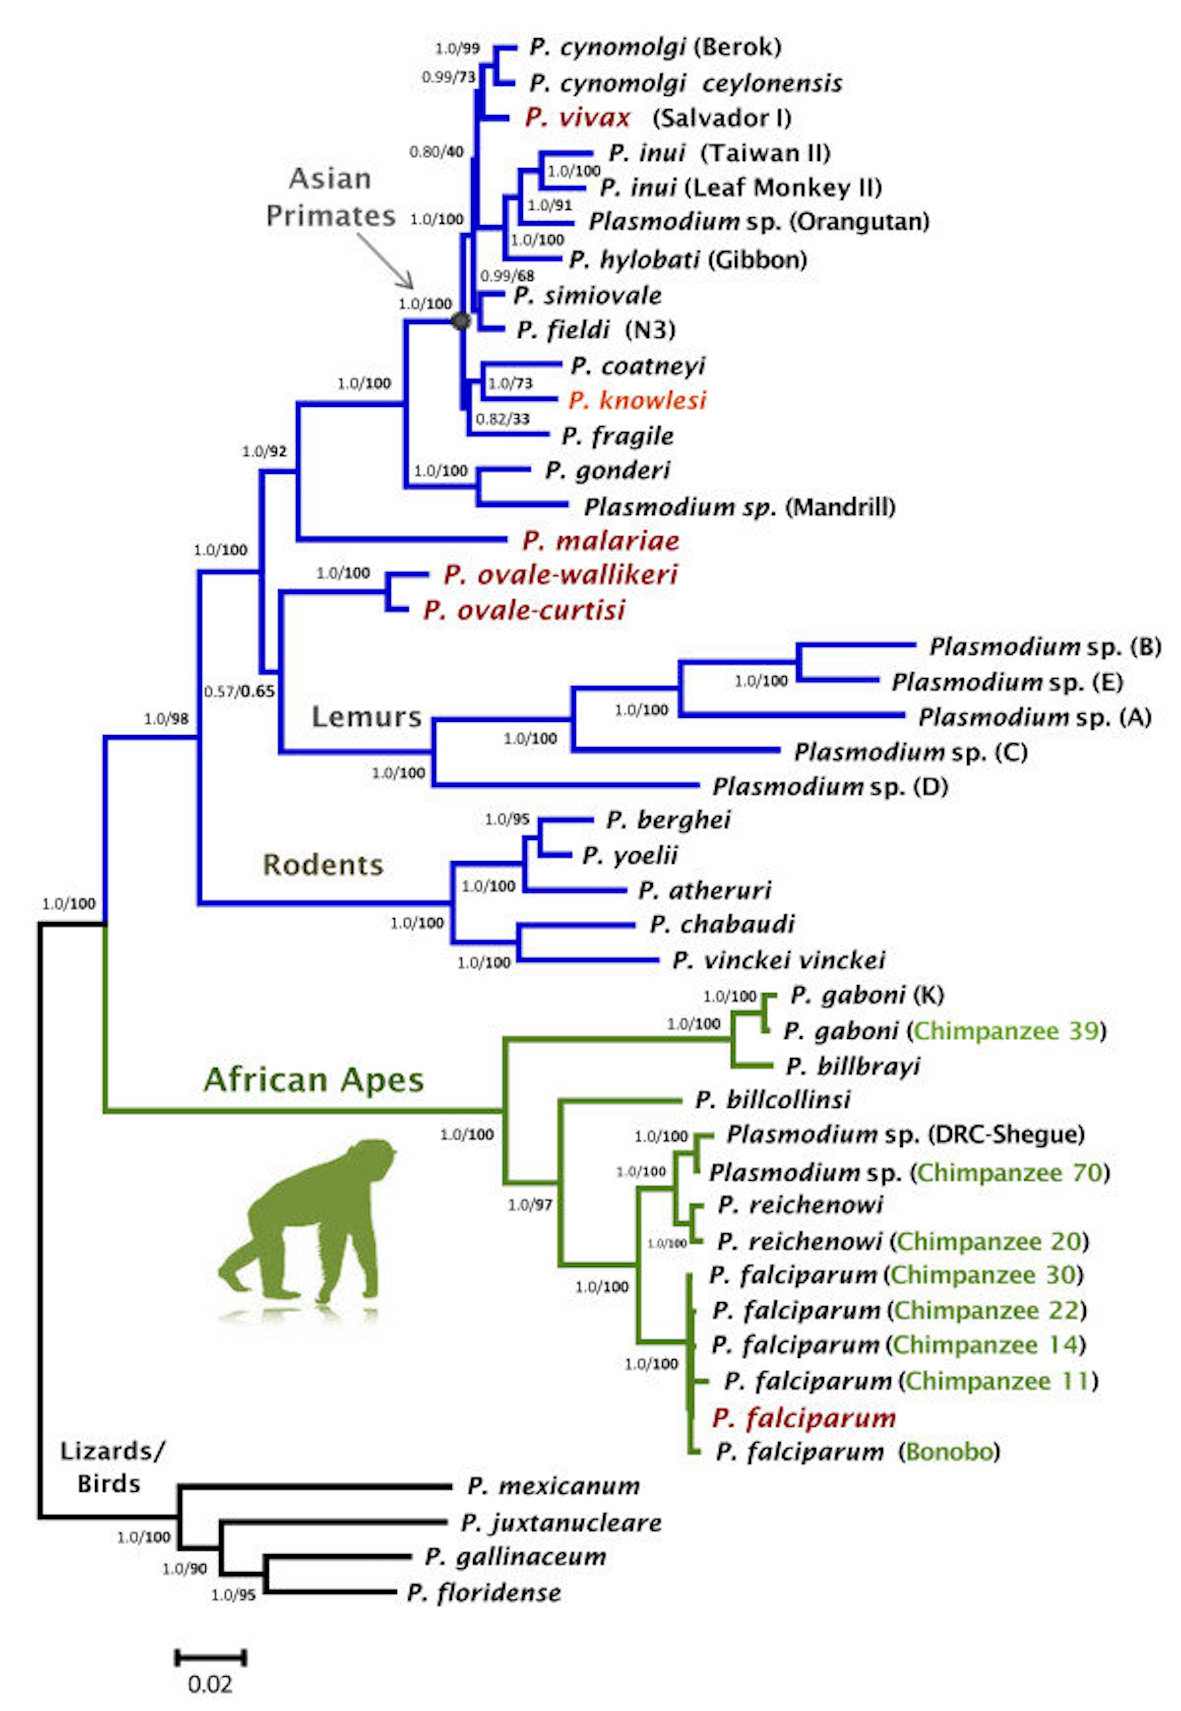
\includegraphics{images/comparative_1.png}

As shown by this figure, there are several closely related species to
\textit{P. falciparum}, of which many have been sequenced. Today, we are
going to use genes identified in the Chimpanzee parasite, \textit{P.
reichenowi}, to annotate genes in \textit{P. falciparum}.

    \hypertarget{challenges-of-protein-to-dna-alignments}{%
\subsection{Challenges of Protein to DNA
Alignments}\label{challenges-of-protein-to-dna-alignments}}

To identify genes in our assembly based on genes from \textit{P.
reichenowi}, we first have to align \textit{P. reichenowi} genes to our
assembly. To do this, we use the protein sequence of \textit{P.
reichenowi} genes and \textit{not} the nucleotide sequence. This is
because the amino acid code is ``degenerate'' and different sets of 3
nucleotides, or a codon, can encode for the same protein as below:

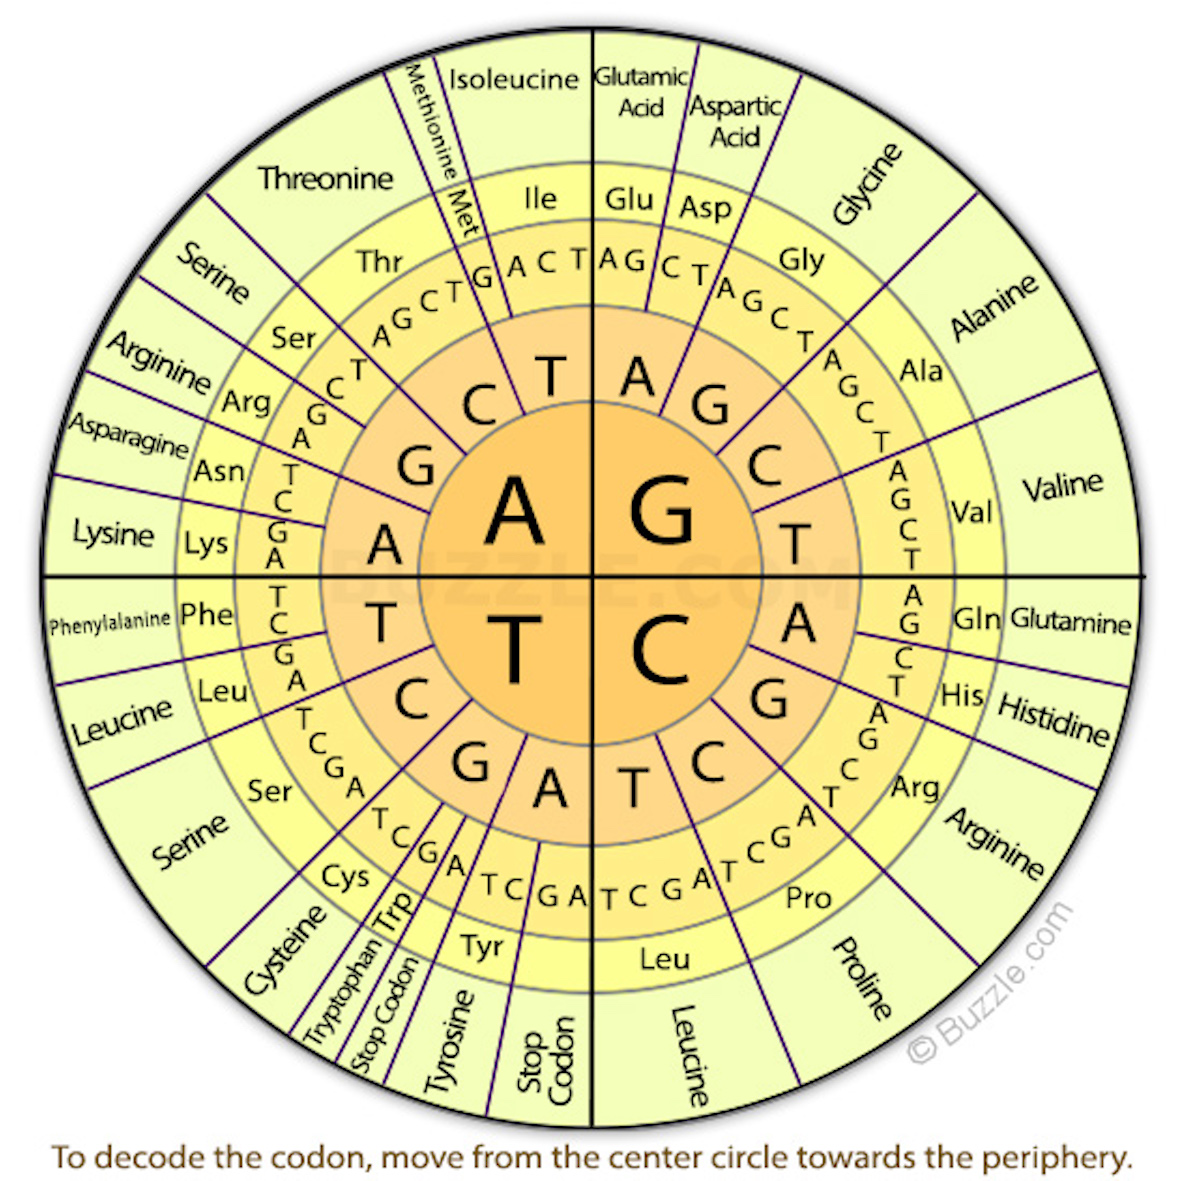
\includegraphics{images/comparative_2.jpg}

In this chart, the first base of a codon is in the innermost circle, the
second base in the next circle, and the final base in the last circle.
In other words, working inside out, TGC codes for the amino acid
Cysteine. This chart also demonstrates how the amino acid code is
``degenerate''. For example, the amino acid threonine can be encoded by
four different codons: ACA, ACT, ACG, or ACC.

This means that closely related organisms can have different nucleotide
sequence, but still have the same amino acid sequence. In the image
below, eventhough \textit{P. falciparum} has an ``A'' at position 9 but
\textit{P. reichenowi} has a ``G'', both specie's proteins have a
threonine amino acid as the third residue:

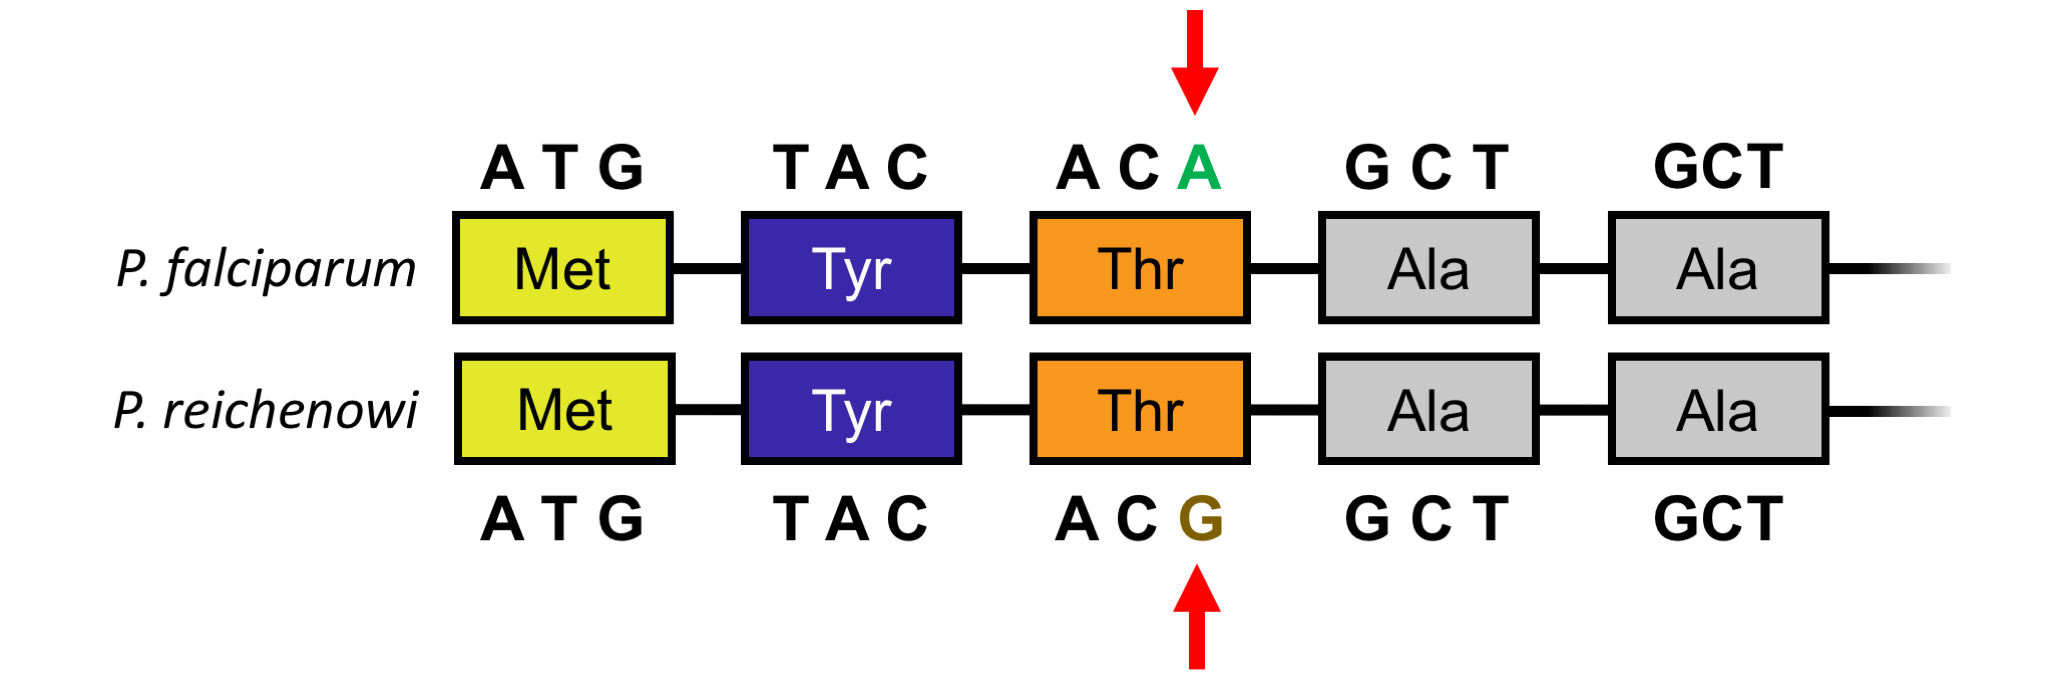
\includegraphics{images/comparative_3.png}

As such, if we use the amino acid sequence of \textit{P. reichenowi} genes
to align to our \textit{P. falciparum} assembly instead of the DNA
sequence, we have more room for error since an amino acid can match
multiple nucleotides. However, this is not a trivial task, as eukaryotic
genes have introns:


\includegraphics{images/comparative_activity_1.png}

\textbf{Questions:}

\begin{enumerate}
\def\labelenumi{\arabic{enumi}.}
\tightlist
\item
  What is difficult about this alignment?
\item
  Did you notice something at the end of the alignment that was not in
  the protein sequence?
\end{enumerate}

Additionally, since the last common ancestor of \textit{P. falciparum} and
\textit{P. reichenowi} new mutations have occured. Thus there will be some
differences in amino acids between the two species:

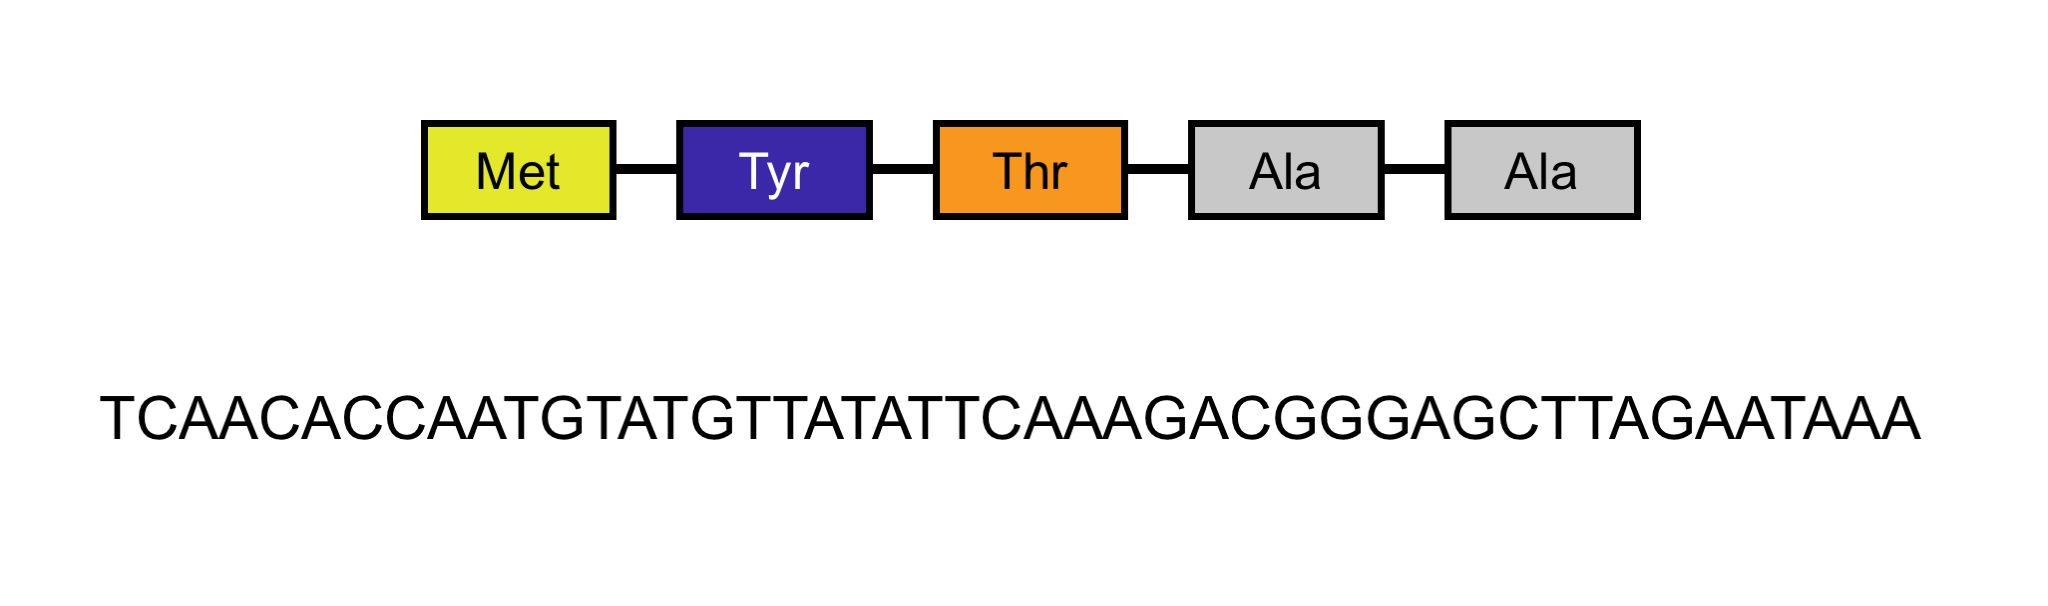
\includegraphics{images/comparative_activity_2.png}

\textbf{Questions:}

\begin{enumerate}
\def\labelenumi{\arabic{enumi}.}
\tightlist
\item
  What was difficult in this example?
\item
  Do you think this is an issue, or is there something biology-related
  going on?
\end{enumerate}

    \hypertarget{aligning-protein-sequences-to-genomes-with-genomethreader}{%
\subsection{Aligning Protein Sequences to Genomes with
GenomeThreader}\label{aligning-protein-sequences-to-genomes-with-genomethreader}}

While our example above was on a very short amino acid sequence, we need
a tool which can perform this basic task for all genes in the \textit{P.
reichenowi} genome across our entire \textit{P. falciparum} assembly. To
do this, we are going to use the tool ``GenomeThreader''. GenomeThreader
is available \href{https://genomethreader.org/}{online} and via
bioconda.

To prepare for this exercise, we have already downloaded all \textit{P.
reichenowi} genes from \href{https://plasmodb.org/plasmo/app/}{PlasmoDB}
and filtered them to genes that will only align to your assembly to save
time. Let's take a look at this file:

    \begin{tcolorbox}[breakable, size=fbox, boxrule=1pt, pad at break*=1mm,colback=cellbackground, colframe=cellborder]
\prompt{In}{incolor}{ }{\boxspacing}
\begin{Verbatim}[commandchars=\\\{\}]
\PY{n}{head} \PY{o}{\PYZhy{}}\PY{n}{n} \PY{l+m+mi}{19} \PY{n}{Preichenowi}\PY{o}{.}\PY{n}{prot}\PY{o}{.}\PY{n}{fa}
\end{Verbatim}
\end{tcolorbox}

    This command will show you the first 19 lines of this file. You will
notice that this file appears similar to the previous .fasta or .fa
files that you have looked at, but now includes more letters. These are
the \href{https://www.bioinformatics.org/sms/iupac.html}{IUPAC amino
acid codes}, and are used to represent all 20 possible amino acids.

If you take a closer look at this file, you may notice the character
\texttt{*}.

\textbf{Question:} What do you think the \texttt{*} character
represents?

Now, we are going to use GenomeThreader (via the \texttt{gth} command)
to align these proteins to your assembly.

    \begin{tcolorbox}[breakable, size=fbox, boxrule=1pt, pad at break*=1mm,colback=cellbackground, colframe=cellborder]
\prompt{In}{incolor}{ }{\boxspacing}
\begin{Verbatim}[commandchars=\\\{\}]
\PY{n}{gth} \PY{o}{\PYZhy{}}\PY{n}{genomic} \PY{n}{PB}\PY{o}{.}\PY{n}{masked}\PY{o}{.}\PY{n}{fasta} \PY{o}{\PYZhy{}}\PY{n}{protein} \PY{n}{Preichenowi}\PY{o}{.}\PY{n}{chr5}\PY{o}{.}\PY{n}{prot}\PY{o}{.}\PY{n}{fa} \PY{o}{\PYZhy{}}\PY{n}{gff3out} \PY{o}{\PYZhy{}}\PY{n}{skipalignmentout} \PY{o}{\PYZhy{}}\PY{n}{paralogs} \PY{o}{\PYZhy{}}\PY{n}{gcmincoverage} \PY{l+m+mi}{80} \PY{o}{\PYZhy{}}\PY{n}{prseedlength} \PY{l+m+mi}{20} \PY{o}{\PYZhy{}}\PY{n}{prminmatchlen} \PY{l+m+mi}{20} \PY{o}{\PYZhy{}}\PY{n}{prhdist} \PY{l+m+mi}{2} \PY{o}{\PYZhy{}}\PY{n}{o} \PY{n}{gth}\PY{o}{.}\PY{n}{gff3} \PY{o}{\PYZhy{}}\PY{n}{finalstopcodon}
\end{Verbatim}
\end{tcolorbox}

    The options above tell genomethreader to:

\begin{itemize}
\tightlist
\item
  \texttt{-gff3out}: print
  \href{https://m.ensembl.org/info/website/upload/gff3.html}{gff3}
  format output (the file \texttt{gth.gff3})
\item
  \texttt{-skipalignmentout}: Do not print anything other than gff3
\item
  \texttt{-paralogs}: Allow the protein sequence to match multiple times
  to our assembly to find genes that are closely related, i.e.~paralogs.
\item
  \texttt{-gcmincoverage\ 80}: Report only proteins which match AT LEAST
  80\% of our assembly
\item
  \texttt{-prseedlength\ 20}, \texttt{-prminmatchlen\ 20}, and
  \texttt{-prhdist\ 2}: Deal with the minimum initial match allowed in
  the ``seed'' of the alignment.
\item
  \texttt{-finalstopcodon}: ensures that each gene is annotated with a
  ``stop''.
\end{itemize}

This command should take a minute or two to run. If it does not complete
or takes too long, you can find a copy of the output in
\texttt{annotation\_backups/}

This file can also be used as the input to Augustus to find genes like
we did above. We don't have enough time today, but feel free to come
back and give it a try! If you want to try, start at section 4.2 with
the commands:

    \begin{tcolorbox}[breakable, size=fbox, boxrule=1pt, pad at break*=1mm,colback=cellbackground, colframe=cellborder]
\prompt{In}{incolor}{ }{\boxspacing}
\begin{Verbatim}[commandchars=\\\{\}]
\PY{n}{gth2gtf}\PY{o}{.}\PY{n}{pl} \PY{n}{gth}\PY{o}{.}\PY{n}{gff3} \PY{n}{bonafide}\PY{o}{.}\PY{n}{gth}\PY{o}{.}\PY{n}{gtf}

\PY{n}{computeFlankingRegion}\PY{o}{.}\PY{n}{pl} \PY{n}{bonafide}\PY{o}{.}\PY{n}{gth}\PY{o}{.}\PY{n}{gtf}
\end{Verbatim}
\end{tcolorbox}

    And proceed through the tutorial from there.

    \hypertarget{examining-and-interpreting-results}{%
\subsection{Examining and Interpreting
Results}\label{examining-and-interpreting-results}}

Now that we have aligned our proteins to our genome assembly, return to
IGV to see if we can learn anything else about that gene we highlighted
at the end of section 4.5. If you closed IGV, see section 4.5 on how to
load your data again.

Now, let's load your new gene ``annotation'' information generated by
GenomeThreader into IGV:

\textbf{Go to \textit{``File -\textgreater{} Load From File''}. Select
``gth.gff3'' and click \textit{``Open''}.}

Now, return to the gene that we previously examined at the end of
section 4.5 by going to the coordinates:

\begin{verbatim}
tig00000001:165,000-171,500
\end{verbatim}

Now, you should see an additional model below your original gene
predictions. It should be named something like ``mRNA21'' - this doesn't
seem very informative! However, if we click the gene model, we should
see an image like the following:

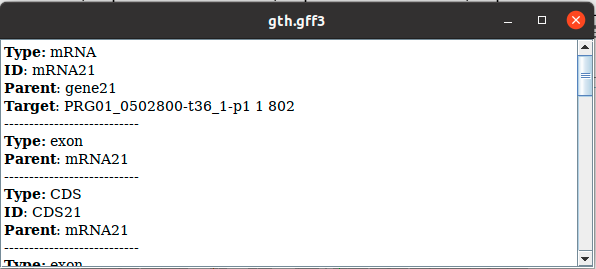
\includegraphics{images/comparative_4.png}

The ``Target'' field tells us the original name of the gene in \textit{P.
reichenowi} that we aligned to our assembly. Now, we are going to use a
web resource to figure out what this gene does. On your desktop open the
web browser.

Once your web browser has loaded, go to the website:

https://plasmodb.org

Being able to query online sequence resources and databases such as
PlasmoDB is an important skill. PlasmoDB contains sequencing data,
protein information, and more for a large number of \textit{Plasmodium}
species. PlasmoDB is part of a larger database, VEuPathDB, which
documents a wide range of eukaryotic parasites such as \textit{P.
falciparum}. While we will only briefly go into PlasmoDB today, we
highly recommend you familiarize yourself with tools such as PlasmoDB.
Other fantastic resources include the
\href{https://genome.ucsc.edu/}{UCSC genome browser} and
\href{https://www.ensembl.org/index.html}{Ensembl} which are dedicated
to providing a wealth of information for hundreds of organisms.

Now, in the search bar at the top of PlasmoDB, enter the first part of
the gene name we found above:


\includegraphics{images/comparative_6.png}

Hit the magnifying glass or ``enter''.

\textbf{Questions:}

\begin{enumerate}
\def\labelenumi{\arabic{enumi}.}
\tightlist
\item
  What is the gene that we identified in IGV?
\item
  Can you name a function of this gene and how did you get the answer?
  \textit{hint: you do not have to use PlasmoDB!}
\end{enumerate}

Congratulations, you have reached the end of the Genome Annotation
tutorial!


    % Add a bibliography block to the postdoc



\end{document}
